% **************************************************************************************************************
% A Classic Thesis Style
% An Homage to The Elements of Typographic Style
%
% Copyright (C) 2011 Andr\'e Miede http://www.miede.de
%
% If you like the style then I would appreciate a postcard. My address 
% can be found in the file ClassicThesis.pdf. A collection of the 
% postcards I received so far is available online at 
% http://postcards.miede.de
%
% License:
% This program is free software; you can redistribute it and/or modify
% it under the terms of the GNU General Public License as published by
% the Free Software Foundation; either version 2 of the License, or
% (at your option) any later version.
%
% This program is distributed in the hope that it will be useful,
% but WITHOUT ANY WARRANTY; without even the implied warranty of
% MERCHANTABILITY or FITNESS FOR A PARTICULAR PURPOSE.  See the
% GNU General Public License for more details.
%
% You should have received a copy of the GNU General Public License
% along with this program; see the file COPYING.  If not, write to
% the Free Software Foundation, Inc., 59 Temple Place - Suite 330,
% Boston, MA 02111-1307, USA.
%
% **************************************************************************************************************
% Note:
%    * You must not use "u etc. in strings/commands that will be spaced out (use \"u or real umlauts instead)
%    * New enumeration (small caps): \begin{aenumerate} \end{aenumerate}
%    * For margin notes: \marginpar or \graffito{}
%    * Do not use bold fonts in this style, it is designed around them
%    * Use tables as in the examples
%    * See classicthesis-preamble.sty for useful commands
% **************************************************************************************************************
% To Do:
%		 * [high] Check this out: http://www.golatex.de/koma-script-warnung-in-verbindung-mit-listings-package-t2058.html
%    * [medium] mathbb in section-titles/chapter-titles => disappears somehow in headlines!!!
% **************************************************************************************************************
\documentclass[ twoside,openright,titlepage,numbers=noenddot,headinclude,%1headlines,% letterpaper a4paper
                footinclude=true,cleardoublepage=empty,abstractoff, % <--- obsolete, remove (todo)
                BCOR=15mm,letterpaper,%=letter,
fontsize=11pt,%11pt,a4paper,%
                ngerman,american,spanish%
                ]{scrreprt}

%********************************************************************
% Note: Make all your adjustments in here
%*******************************************************
% ****************************************************************************************************
% classicthesis-config.tex 
% formerly known as loadpackages.sty, classicthesis-ldpkg.sty, and classicthesis-preamble.sty 
% Use it at the beginning of your ClassicThesis.tex, or as a LaTeX Preamble 
% in your ClassicThesis.{tex,lyx} with % ****************************************************************************************************
% classicthesis-config.tex 
% formerly known as loadpackages.sty, classicthesis-ldpkg.sty, and classicthesis-preamble.sty 
% Use it at the beginning of your ClassicThesis.tex, or as a LaTeX Preamble 
% in your ClassicThesis.{tex,lyx} with % ****************************************************************************************************
% classicthesis-config.tex 
% formerly known as loadpackages.sty, classicthesis-ldpkg.sty, and classicthesis-preamble.sty 
% Use it at the beginning of your ClassicThesis.tex, or as a LaTeX Preamble 
% in your ClassicThesis.{tex,lyx} with \input{classicthesis-config}
% ****************************************************************************************************  
% If you like the classicthesis, then I would appreciate a postcard. 
% My address can be found in the file ClassicThesis.pdf. A collection 
% of the postcards I received so far is available online at 
% http://postcards.miede.de
% ****************************************************************************************************

% ****************************************************************************************************
% 1. Configure classicthesis for your needs here, e.g., remove "drafting" below 
% in order to deactivate the time-stamp on the pages
% ****************************************************************************************************
\PassOptionsToPackage{eulerchapternumbers,%listings,
				%drafting,%
				 pdfspacing,%floatperchapter,
				linedheaders,%
				tocaligned,dottedtoc,
				 subfig,beramono%,eulermath
}{classicthesis}										
% ********************************************************************
% Available options for classicthesis.sty 
% (see ClassicThesis.pdf for more information):
% drafting
% parts nochapters linedheaders
% eulerchapternumbers beramono eulermath pdfspacing minionprospacing
% tocaligned dottedtoc manychapters
% listings floatperchapter subfig
% ********************************************************************

% ********************************************************************
% Triggers for this config
% ******************************************************************** 
\usepackage{ifthen}
\newboolean{enable-backrefs} % enable backrefs in the bibliography
\setboolean{enable-backrefs}{true} % true false
% ****************************************************************************************************


% ****************************************************************************************************
% 2. Personal data and user ad-hoc commands
% ****************************************************************************************************
\newcommand{\myTitle}{Modelos semicontinuos de redes de se\~nalizaci\'on en el espermatozoide de erizo de mar\xspace}
\newcommand{\mySubtitle}{\xspace}
\newcommand{\myDegree}{Maestro en Ciencias}
\newcommand{\myName}{Lic. en C. Rafael Verduzco V\'azquez\xspace}
\newcommand{\myProf}{Dr. Gustavo Mart\'inez Mekler\xspace}
\newcommand{\myOtherProf}{Dr. Maximino Aldana González\xspace}
\newcommand{\myFirstRevisor}{Dr. Hern\'an Larralde Ridaura\xspace}
\newcommand{\mySecondRevisor}{Dr. Jos\'e D\'iaz Escudero\xspace}
\newcommand{\myThirdRevisor}{Dr. Ra\'ul Rechtman Schrenzel\xspace}
\newcommand{\myFourthRevisor}{Dr. Ra\'ul Salgado Garc\'ia\xspace}
\newcommand{\mySupervisor}{Put name here\xspace}
\newcommand{\myFaculty}{Facultad de Ciencias\xspace}
\newcommand{\myDepartment}{Put data here\xspace}
\newcommand{\myUni}{Universidad Aut\'onoma del Estado de Morelos\xspace}
\newcommand{\myLocation}{Kornbach\xspace}
\newcommand{\myTime}{Octubre de 2012\xspace}
\newcommand{\myVersion}{\xspace}

% ********************************************************************
% Setup, finetuning, and useful commands
% ********************************************************************
\newcounter{dummy} % necessary for correct hyperlinks (to index, bib, etc.)
\newlength{\abcd} % for ab..z string length calculation
\providecommand{\mLyX}{L\kern-.1667em\lower.25em\hbox{Y}\kern-.125emX\@}
\newcommand{\ie}{i.\,e.}
\newcommand{\Ie}{I.\,e.}
\newcommand{\eg}{e.\,g.}
\newcommand{\Eg}{E.\,g.} 
% ****************************************************************************************************


% ****************************************************************************************************
% 3. Loading some handy packages
% ****************************************************************************************************
% ******************************************************************** 
% Packages with options that might require adjustments
% ******************************************************************** 
\PassOptionsToPackage{utf8}{inputenc}	% latin9 (ISO-8859-9) = latin1+"Euro sign"
 \usepackage{inputenc}				


\PassOptionsToPackage{square,numbers}{natbib}
 \usepackage{natbib}	
 
%\PassOptionsToPackage{ngerman,american}{babel}   % change this to your language(s)
% Spanish languages need extra options in order to work with this template
\PassOptionsToPackage{spanish,es-lcroman,mexico}{babel}
 \usepackage{babel}					

%% Added by me =P
%\PassOptionsToPackage{fixlanguage}{babelbib}
% \usepackage{babelbib}

\PassOptionsToPackage{fleqn}{amsmath}		% math environments and more by the AMS 
 \usepackage{amsmath}

% ******************************************************************** 
% General useful packages
% ******************************************************************** 
\PassOptionsToPackage{T1}{fontenc} % T2A for cyrillics
	\usepackage{fontenc}                 
\usepackage{xspace} % to get the spacing after macros right  
\usepackage{mparhack} % get marginpar right
\usepackage{fixltx2e} % fixes some LaTeX stuff 
\PassOptionsToPackage{printonlyused,smaller}{acronym}
	\usepackage{acronym} % nice macros for handling all acronyms in the thesis
%\renewcommand*{\acsfont}[1]{\textssc{#1}} % for MinionPro
\renewcommand{\bflabel}[1]{{#1}\hfill} % fix the list of acronyms
% ****************************************************************************************************


% ****************************************************************************************************
% 4. Setup floats: tables, (sub)figures, and captions
% ****************************************************************************************************
\usepackage{tabularx} % better tables
	\setlength{\extrarowheight}{3pt} % increase table row height
\newcommand{\tableheadline}[1]{\multicolumn{1}{c}{\spacedlowsmallcaps{#1}}}
\newcommand{\myfloatalign}{\centering} % to be used with each float for alignment
\usepackage{caption}
\captionsetup{format=hang,font=small}
\usepackage{subfig}  
% ****************************************************************************************************


% ****************************************************************************************************
% 5. Setup code listings
% ****************************************************************************************************
\usepackage{listings} 
%\lstset{emph={trueIndex,root},emphstyle=\color{BlueViolet}}%\underbar} % for special keywords
\lstset{language=[ANSI]C,%[LaTeX]Tex,%C++,
    keywordstyle=\color{RoyalBlue},%\bfseries,
    basicstyle=\small\ttfamily,
    identifierstyle=\color{Maroon},
    commentstyle=\color{Green}\ttfamily,
    stringstyle=\rmfamily,
    numbers=none,%left,%
    numberstyle=\scriptsize,%\tiny
    stepnumber=5,
    numbersep=8pt,
    showstringspaces=false,
    breaklines=true,
    frameround=ftff,
    frame=single,
    belowcaptionskip=.75\baselineskip
    %frame=L
} 
% ****************************************************************************************************    		   


% ****************************************************************************************************
% 6. PDFLaTeX, hyperreferences and citation backreferences
% ****************************************************************************************************
% ********************************************************************
% Using PDFLaTeX
% ********************************************************************
\PassOptionsToPackage{pdftex,hyperfootnotes=false,pdfpagelabels}{hyperref}
	\usepackage{hyperref}  % backref linktocpage pagebackref
\pdfcompresslevel=9
\pdfadjustspacing=1 
\PassOptionsToPackage{pdftex}{graphicx}
	\usepackage{graphicx} 

% ********************************************************************
% Setup the style of the backrefs from the bibliography
% (translate the options to any language you use)
% ********************************************************************
\newcommand{\backrefnotcitedstring}{\relax}%(Not cited.)
\newcommand{\backrefcitedsinglestring}[1]{(Citado en la p\'agina~#1.)}
\newcommand{\backrefcitedmultistring}[1]{(Citado en las p\'aginas~#1.)}
\ifthenelse{\boolean{enable-backrefs}}%
{%
		\PassOptionsToPackage{hyperpageref}{backref}
		\usepackage{backref} % to be loaded after hyperref package 
		   \renewcommand{\backreftwosep}{ y~} % separate 2 pages
		   \renewcommand{\backreflastsep}{, y~} % separate last of longer list
		   \renewcommand*{\backref}[1]{}  % disable standard
		   \renewcommand*{\backrefalt}[4]{% detailed backref
		      \ifcase #1 %
		         \backrefnotcitedstring%
		      \or%
		         \backrefcitedsinglestring{#2}%
		      \else%
		         \backrefcitedmultistring{#2}%
		      \fi}%
}{\relax}    

% ********************************************************************
% Hyperreferences
% ********************************************************************
\hypersetup{%
    %draft,	% = no hyperlinking at all (useful in b/w printouts)
    colorlinks=true, linktocpage=true, pdfstartpage=3, pdfstartview=FitV,%
    % uncomment the following line if you want to have black links (e.g., for printing)
    %colorlinks=false, linktocpage=false, pdfborder={0 0 0}, pdfstartpage=3, pdfstartview=FitV,% 
    breaklinks=true, pdfpagemode=UseNone, pageanchor=true, pdfpagemode=UseOutlines,%
    plainpages=false, bookmarksnumbered, bookmarksopen=true, bookmarksopenlevel=1,%
    hypertexnames=true, pdfhighlight=/O,%nesting=true,%frenchlinks,%
    urlcolor=webbrown, linkcolor=RoyalBlue, citecolor=webgreen, %pagecolor=RoyalBlue,%
    %urlcolor=Black, linkcolor=Black, citecolor=Black, %pagecolor=Black,%
    pdftitle={\myTitle},%
    pdfauthor={\textcopyright\ \myName, \myUni, \myFaculty},%
    pdfsubject={},%
    pdfkeywords={},%
    pdfcreator={pdfLaTeX},%
    pdfproducer={LaTeX with hyperref and classicthesis}%
}   

% ********************************************************************
% Setup autoreferences
% ********************************************************************
% There are some issues regarding autorefnames
% http://www.ureader.de/msg/136221647.aspx
% http://www.tex.ac.uk/cgi-bin/texfaq2html?label=latexwords
% you have to redefine the makros for the 
% language you use, e.g., american, ngerman
% (as chosen when loading babel/AtBeginDocument)
% ********************************************************************
\makeatletter
\@ifpackageloaded{babel}%
    {%
       \addto\extrasamerican{%
					\renewcommand*{\figureautorefname}{Figure}%
					\renewcommand*{\tableautorefname}{Table}%
					\renewcommand*{\partautorefname}{Part}%
					\renewcommand*{\chapterautorefname}{Chapter}%
					\renewcommand*{\sectionautorefname}{Section}%
					\renewcommand*{\subsectionautorefname}{Section}%
					\renewcommand*{\subsubsectionautorefname}{Section}% 	
				}%
       \addto\extrasngerman{% 
					\renewcommand*{\paragraphautorefname}{Absatz}%
					\renewcommand*{\subparagraphautorefname}{Unterabsatz}%
					\renewcommand*{\footnoteautorefname}{Fu\"snote}%
					\renewcommand*{\FancyVerbLineautorefname}{Zeile}%
					\renewcommand*{\theoremautorefname}{Theorem}%
					\renewcommand*{\appendixautorefname}{Anhang}%
					\renewcommand*{\equationautorefname}{Gleichung}%        
					\renewcommand*{\itemautorefname}{Punkt}%
				}%	
			% Fix to getting autorefs for subfigures right (thanks to Belinda Vogt for changing the definition)
			\providecommand{\subfigureautorefname}{\figureautorefname}%  			
    }{\relax}
\makeatother


% ****************************************************************************************************
% 7. Last calls before the bar closes
% ****************************************************************************************************
% ********************************************************************
% Development Stuff
% ********************************************************************
\listfiles
%\PassOptionsToPackage{l2tabu,orthodox,abort}{nag}
%	\usepackage{nag}
%\PassOptionsToPackage{warning, all}{onlyamsmath}
%	\usepackage{onlyamsmath}'

% ********************************************************************
% Last, but not least...
% ********************************************************************
\usepackage{classicthesis} 
% ****************************************************************************************************


% ****************************************************************************************************
% 8. Further adjustments (experimental)
% ****************************************************************************************************
% ********************************************************************
% Changing the text area
% ********************************************************************
%\linespread{1.05} % a bit more for Palatino
%\areaset[current]{312pt}{761pt} % 686 (factor 2.2) + 33 head + 42 head \the\footskip
%\setlength{\marginparwidth}{7em}%
%\setlength{\marginparsep}{2em}%

% ********************************************************************
% Using different fonts
% ********************************************************************
\usepackage[oldstylenums]{kpfonts} % oldstyle notextcomp
%\usepackage[osf]{libertine}
%\usepackage{hfoldsty} % Computer Modern with osf
%\usepackage[light,condensed,math]{iwona}
%\renewcommand{\sfdefault}{iwona}
%\usepackage{lmodern} % <-- no osf support :-(
%\usepackage[urw-garamond]{mathdesign} <-- no osf support :-(
% ****************************************************************************************************

% ****************************************************************************************************  
% If you like the classicthesis, then I would appreciate a postcard. 
% My address can be found in the file ClassicThesis.pdf. A collection 
% of the postcards I received so far is available online at 
% http://postcards.miede.de
% ****************************************************************************************************

% ****************************************************************************************************
% 1. Configure classicthesis for your needs here, e.g., remove "drafting" below 
% in order to deactivate the time-stamp on the pages
% ****************************************************************************************************
\PassOptionsToPackage{eulerchapternumbers,%listings,
				%drafting,%
				 pdfspacing,%floatperchapter,
				linedheaders,%
				tocaligned,dottedtoc,
				 subfig,beramono%,eulermath
}{classicthesis}										
% ********************************************************************
% Available options for classicthesis.sty 
% (see ClassicThesis.pdf for more information):
% drafting
% parts nochapters linedheaders
% eulerchapternumbers beramono eulermath pdfspacing minionprospacing
% tocaligned dottedtoc manychapters
% listings floatperchapter subfig
% ********************************************************************

% ********************************************************************
% Triggers for this config
% ******************************************************************** 
\usepackage{ifthen}
\newboolean{enable-backrefs} % enable backrefs in the bibliography
\setboolean{enable-backrefs}{true} % true false
% ****************************************************************************************************


% ****************************************************************************************************
% 2. Personal data and user ad-hoc commands
% ****************************************************************************************************
\newcommand{\myTitle}{Modelos semicontinuos de redes de se\~nalizaci\'on en el espermatozoide de erizo de mar\xspace}
\newcommand{\mySubtitle}{\xspace}
\newcommand{\myDegree}{Maestro en Ciencias}
\newcommand{\myName}{Lic. en C. Rafael Verduzco V\'azquez\xspace}
\newcommand{\myProf}{Dr. Gustavo Mart\'inez Mekler\xspace}
\newcommand{\myOtherProf}{Dr. Maximino Aldana González\xspace}
\newcommand{\myFirstRevisor}{Dr. Hern\'an Larralde Ridaura\xspace}
\newcommand{\mySecondRevisor}{Dr. Jos\'e D\'iaz Escudero\xspace}
\newcommand{\myThirdRevisor}{Dr. Ra\'ul Rechtman Schrenzel\xspace}
\newcommand{\myFourthRevisor}{Dr. Ra\'ul Salgado Garc\'ia\xspace}
\newcommand{\mySupervisor}{Put name here\xspace}
\newcommand{\myFaculty}{Facultad de Ciencias\xspace}
\newcommand{\myDepartment}{Put data here\xspace}
\newcommand{\myUni}{Universidad Aut\'onoma del Estado de Morelos\xspace}
\newcommand{\myLocation}{Kornbach\xspace}
\newcommand{\myTime}{Octubre de 2012\xspace}
\newcommand{\myVersion}{\xspace}

% ********************************************************************
% Setup, finetuning, and useful commands
% ********************************************************************
\newcounter{dummy} % necessary for correct hyperlinks (to index, bib, etc.)
\newlength{\abcd} % for ab..z string length calculation
\providecommand{\mLyX}{L\kern-.1667em\lower.25em\hbox{Y}\kern-.125emX\@}
\newcommand{\ie}{i.\,e.}
\newcommand{\Ie}{I.\,e.}
\newcommand{\eg}{e.\,g.}
\newcommand{\Eg}{E.\,g.} 
% ****************************************************************************************************


% ****************************************************************************************************
% 3. Loading some handy packages
% ****************************************************************************************************
% ******************************************************************** 
% Packages with options that might require adjustments
% ******************************************************************** 
\PassOptionsToPackage{utf8}{inputenc}	% latin9 (ISO-8859-9) = latin1+"Euro sign"
 \usepackage{inputenc}				


\PassOptionsToPackage{square,numbers}{natbib}
 \usepackage{natbib}	
 
%\PassOptionsToPackage{ngerman,american}{babel}   % change this to your language(s)
% Spanish languages need extra options in order to work with this template
\PassOptionsToPackage{spanish,es-lcroman,mexico}{babel}
 \usepackage{babel}					

%% Added by me =P
%\PassOptionsToPackage{fixlanguage}{babelbib}
% \usepackage{babelbib}

\PassOptionsToPackage{fleqn}{amsmath}		% math environments and more by the AMS 
 \usepackage{amsmath}

% ******************************************************************** 
% General useful packages
% ******************************************************************** 
\PassOptionsToPackage{T1}{fontenc} % T2A for cyrillics
	\usepackage{fontenc}                 
\usepackage{xspace} % to get the spacing after macros right  
\usepackage{mparhack} % get marginpar right
\usepackage{fixltx2e} % fixes some LaTeX stuff 
\PassOptionsToPackage{printonlyused,smaller}{acronym}
	\usepackage{acronym} % nice macros for handling all acronyms in the thesis
%\renewcommand*{\acsfont}[1]{\textssc{#1}} % for MinionPro
\renewcommand{\bflabel}[1]{{#1}\hfill} % fix the list of acronyms
% ****************************************************************************************************


% ****************************************************************************************************
% 4. Setup floats: tables, (sub)figures, and captions
% ****************************************************************************************************
\usepackage{tabularx} % better tables
	\setlength{\extrarowheight}{3pt} % increase table row height
\newcommand{\tableheadline}[1]{\multicolumn{1}{c}{\spacedlowsmallcaps{#1}}}
\newcommand{\myfloatalign}{\centering} % to be used with each float for alignment
\usepackage{caption}
\captionsetup{format=hang,font=small}
\usepackage{subfig}  
% ****************************************************************************************************


% ****************************************************************************************************
% 5. Setup code listings
% ****************************************************************************************************
\usepackage{listings} 
%\lstset{emph={trueIndex,root},emphstyle=\color{BlueViolet}}%\underbar} % for special keywords
\lstset{language=[ANSI]C,%[LaTeX]Tex,%C++,
    keywordstyle=\color{RoyalBlue},%\bfseries,
    basicstyle=\small\ttfamily,
    identifierstyle=\color{Maroon},
    commentstyle=\color{Green}\ttfamily,
    stringstyle=\rmfamily,
    numbers=none,%left,%
    numberstyle=\scriptsize,%\tiny
    stepnumber=5,
    numbersep=8pt,
    showstringspaces=false,
    breaklines=true,
    frameround=ftff,
    frame=single,
    belowcaptionskip=.75\baselineskip
    %frame=L
} 
% ****************************************************************************************************    		   


% ****************************************************************************************************
% 6. PDFLaTeX, hyperreferences and citation backreferences
% ****************************************************************************************************
% ********************************************************************
% Using PDFLaTeX
% ********************************************************************
\PassOptionsToPackage{pdftex,hyperfootnotes=false,pdfpagelabels}{hyperref}
	\usepackage{hyperref}  % backref linktocpage pagebackref
\pdfcompresslevel=9
\pdfadjustspacing=1 
\PassOptionsToPackage{pdftex}{graphicx}
	\usepackage{graphicx} 

% ********************************************************************
% Setup the style of the backrefs from the bibliography
% (translate the options to any language you use)
% ********************************************************************
\newcommand{\backrefnotcitedstring}{\relax}%(Not cited.)
\newcommand{\backrefcitedsinglestring}[1]{(Citado en la p\'agina~#1.)}
\newcommand{\backrefcitedmultistring}[1]{(Citado en las p\'aginas~#1.)}
\ifthenelse{\boolean{enable-backrefs}}%
{%
		\PassOptionsToPackage{hyperpageref}{backref}
		\usepackage{backref} % to be loaded after hyperref package 
		   \renewcommand{\backreftwosep}{ y~} % separate 2 pages
		   \renewcommand{\backreflastsep}{, y~} % separate last of longer list
		   \renewcommand*{\backref}[1]{}  % disable standard
		   \renewcommand*{\backrefalt}[4]{% detailed backref
		      \ifcase #1 %
		         \backrefnotcitedstring%
		      \or%
		         \backrefcitedsinglestring{#2}%
		      \else%
		         \backrefcitedmultistring{#2}%
		      \fi}%
}{\relax}    

% ********************************************************************
% Hyperreferences
% ********************************************************************
\hypersetup{%
    %draft,	% = no hyperlinking at all (useful in b/w printouts)
    colorlinks=true, linktocpage=true, pdfstartpage=3, pdfstartview=FitV,%
    % uncomment the following line if you want to have black links (e.g., for printing)
    %colorlinks=false, linktocpage=false, pdfborder={0 0 0}, pdfstartpage=3, pdfstartview=FitV,% 
    breaklinks=true, pdfpagemode=UseNone, pageanchor=true, pdfpagemode=UseOutlines,%
    plainpages=false, bookmarksnumbered, bookmarksopen=true, bookmarksopenlevel=1,%
    hypertexnames=true, pdfhighlight=/O,%nesting=true,%frenchlinks,%
    urlcolor=webbrown, linkcolor=RoyalBlue, citecolor=webgreen, %pagecolor=RoyalBlue,%
    %urlcolor=Black, linkcolor=Black, citecolor=Black, %pagecolor=Black,%
    pdftitle={\myTitle},%
    pdfauthor={\textcopyright\ \myName, \myUni, \myFaculty},%
    pdfsubject={},%
    pdfkeywords={},%
    pdfcreator={pdfLaTeX},%
    pdfproducer={LaTeX with hyperref and classicthesis}%
}   

% ********************************************************************
% Setup autoreferences
% ********************************************************************
% There are some issues regarding autorefnames
% http://www.ureader.de/msg/136221647.aspx
% http://www.tex.ac.uk/cgi-bin/texfaq2html?label=latexwords
% you have to redefine the makros for the 
% language you use, e.g., american, ngerman
% (as chosen when loading babel/AtBeginDocument)
% ********************************************************************
\makeatletter
\@ifpackageloaded{babel}%
    {%
       \addto\extrasamerican{%
					\renewcommand*{\figureautorefname}{Figure}%
					\renewcommand*{\tableautorefname}{Table}%
					\renewcommand*{\partautorefname}{Part}%
					\renewcommand*{\chapterautorefname}{Chapter}%
					\renewcommand*{\sectionautorefname}{Section}%
					\renewcommand*{\subsectionautorefname}{Section}%
					\renewcommand*{\subsubsectionautorefname}{Section}% 	
				}%
       \addto\extrasngerman{% 
					\renewcommand*{\paragraphautorefname}{Absatz}%
					\renewcommand*{\subparagraphautorefname}{Unterabsatz}%
					\renewcommand*{\footnoteautorefname}{Fu\"snote}%
					\renewcommand*{\FancyVerbLineautorefname}{Zeile}%
					\renewcommand*{\theoremautorefname}{Theorem}%
					\renewcommand*{\appendixautorefname}{Anhang}%
					\renewcommand*{\equationautorefname}{Gleichung}%        
					\renewcommand*{\itemautorefname}{Punkt}%
				}%	
			% Fix to getting autorefs for subfigures right (thanks to Belinda Vogt for changing the definition)
			\providecommand{\subfigureautorefname}{\figureautorefname}%  			
    }{\relax}
\makeatother


% ****************************************************************************************************
% 7. Last calls before the bar closes
% ****************************************************************************************************
% ********************************************************************
% Development Stuff
% ********************************************************************
\listfiles
%\PassOptionsToPackage{l2tabu,orthodox,abort}{nag}
%	\usepackage{nag}
%\PassOptionsToPackage{warning, all}{onlyamsmath}
%	\usepackage{onlyamsmath}'

% ********************************************************************
% Last, but not least...
% ********************************************************************
\usepackage{classicthesis} 
% ****************************************************************************************************


% ****************************************************************************************************
% 8. Further adjustments (experimental)
% ****************************************************************************************************
% ********************************************************************
% Changing the text area
% ********************************************************************
%\linespread{1.05} % a bit more for Palatino
%\areaset[current]{312pt}{761pt} % 686 (factor 2.2) + 33 head + 42 head \the\footskip
%\setlength{\marginparwidth}{7em}%
%\setlength{\marginparsep}{2em}%

% ********************************************************************
% Using different fonts
% ********************************************************************
\usepackage[oldstylenums]{kpfonts} % oldstyle notextcomp
%\usepackage[osf]{libertine}
%\usepackage{hfoldsty} % Computer Modern with osf
%\usepackage[light,condensed,math]{iwona}
%\renewcommand{\sfdefault}{iwona}
%\usepackage{lmodern} % <-- no osf support :-(
%\usepackage[urw-garamond]{mathdesign} <-- no osf support :-(
% ****************************************************************************************************

% ****************************************************************************************************  
% If you like the classicthesis, then I would appreciate a postcard. 
% My address can be found in the file ClassicThesis.pdf. A collection 
% of the postcards I received so far is available online at 
% http://postcards.miede.de
% ****************************************************************************************************

% ****************************************************************************************************
% 1. Configure classicthesis for your needs here, e.g., remove "drafting" below 
% in order to deactivate the time-stamp on the pages
% ****************************************************************************************************
\PassOptionsToPackage{eulerchapternumbers,%listings,
				%drafting,%
				 pdfspacing,%floatperchapter,
				linedheaders,%
				tocaligned,dottedtoc,
				 subfig,beramono%,eulermath
}{classicthesis}										
% ********************************************************************
% Available options for classicthesis.sty 
% (see ClassicThesis.pdf for more information):
% drafting
% parts nochapters linedheaders
% eulerchapternumbers beramono eulermath pdfspacing minionprospacing
% tocaligned dottedtoc manychapters
% listings floatperchapter subfig
% ********************************************************************

% ********************************************************************
% Triggers for this config
% ******************************************************************** 
\usepackage{ifthen}
\newboolean{enable-backrefs} % enable backrefs in the bibliography
\setboolean{enable-backrefs}{true} % true false
% ****************************************************************************************************


% ****************************************************************************************************
% 2. Personal data and user ad-hoc commands
% ****************************************************************************************************
\newcommand{\myTitle}{Modelos semicontinuos de redes de se\~nalizaci\'on en el espermatozoide de erizo de mar\xspace}
\newcommand{\mySubtitle}{\xspace}
\newcommand{\myDegree}{Maestro en Ciencias}
\newcommand{\myName}{Lic. en C. Rafael Verduzco V\'azquez\xspace}
\newcommand{\myProf}{Dr. Gustavo Mart\'inez Mekler\xspace}
\newcommand{\myOtherProf}{Dr. Maximino Aldana González\xspace}
\newcommand{\myFirstRevisor}{Dr. Hern\'an Larralde Ridaura\xspace}
\newcommand{\mySecondRevisor}{Dr. Jos\'e D\'iaz Escudero\xspace}
\newcommand{\myThirdRevisor}{Dr. Ra\'ul Rechtman Schrenzel\xspace}
\newcommand{\myFourthRevisor}{Dr. Ra\'ul Salgado Garc\'ia\xspace}
\newcommand{\mySupervisor}{Put name here\xspace}
\newcommand{\myFaculty}{Facultad de Ciencias\xspace}
\newcommand{\myDepartment}{Put data here\xspace}
\newcommand{\myUni}{Universidad Aut\'onoma del Estado de Morelos\xspace}
\newcommand{\myLocation}{Kornbach\xspace}
\newcommand{\myTime}{Octubre de 2012\xspace}
\newcommand{\myVersion}{\xspace}

% ********************************************************************
% Setup, finetuning, and useful commands
% ********************************************************************
\newcounter{dummy} % necessary for correct hyperlinks (to index, bib, etc.)
\newlength{\abcd} % for ab..z string length calculation
\providecommand{\mLyX}{L\kern-.1667em\lower.25em\hbox{Y}\kern-.125emX\@}
\newcommand{\ie}{i.\,e.}
\newcommand{\Ie}{I.\,e.}
\newcommand{\eg}{e.\,g.}
\newcommand{\Eg}{E.\,g.} 
% ****************************************************************************************************


% ****************************************************************************************************
% 3. Loading some handy packages
% ****************************************************************************************************
% ******************************************************************** 
% Packages with options that might require adjustments
% ******************************************************************** 
\PassOptionsToPackage{utf8}{inputenc}	% latin9 (ISO-8859-9) = latin1+"Euro sign"
 \usepackage{inputenc}				


\PassOptionsToPackage{square,numbers}{natbib}
 \usepackage{natbib}	
 
%\PassOptionsToPackage{ngerman,american}{babel}   % change this to your language(s)
% Spanish languages need extra options in order to work with this template
\PassOptionsToPackage{spanish,es-lcroman,mexico}{babel}
 \usepackage{babel}					

%% Added by me =P
%\PassOptionsToPackage{fixlanguage}{babelbib}
% \usepackage{babelbib}

\PassOptionsToPackage{fleqn}{amsmath}		% math environments and more by the AMS 
 \usepackage{amsmath}

% ******************************************************************** 
% General useful packages
% ******************************************************************** 
\PassOptionsToPackage{T1}{fontenc} % T2A for cyrillics
	\usepackage{fontenc}                 
\usepackage{xspace} % to get the spacing after macros right  
\usepackage{mparhack} % get marginpar right
\usepackage{fixltx2e} % fixes some LaTeX stuff 
\PassOptionsToPackage{printonlyused,smaller}{acronym}
	\usepackage{acronym} % nice macros for handling all acronyms in the thesis
%\renewcommand*{\acsfont}[1]{\textssc{#1}} % for MinionPro
\renewcommand{\bflabel}[1]{{#1}\hfill} % fix the list of acronyms
% ****************************************************************************************************


% ****************************************************************************************************
% 4. Setup floats: tables, (sub)figures, and captions
% ****************************************************************************************************
\usepackage{tabularx} % better tables
	\setlength{\extrarowheight}{3pt} % increase table row height
\newcommand{\tableheadline}[1]{\multicolumn{1}{c}{\spacedlowsmallcaps{#1}}}
\newcommand{\myfloatalign}{\centering} % to be used with each float for alignment
\usepackage{caption}
\captionsetup{format=hang,font=small}
\usepackage{subfig}  
% ****************************************************************************************************


% ****************************************************************************************************
% 5. Setup code listings
% ****************************************************************************************************
\usepackage{listings} 
%\lstset{emph={trueIndex,root},emphstyle=\color{BlueViolet}}%\underbar} % for special keywords
\lstset{language=[ANSI]C,%[LaTeX]Tex,%C++,
    keywordstyle=\color{RoyalBlue},%\bfseries,
    basicstyle=\small\ttfamily,
    identifierstyle=\color{Maroon},
    commentstyle=\color{Green}\ttfamily,
    stringstyle=\rmfamily,
    numbers=none,%left,%
    numberstyle=\scriptsize,%\tiny
    stepnumber=5,
    numbersep=8pt,
    showstringspaces=false,
    breaklines=true,
    frameround=ftff,
    frame=single,
    belowcaptionskip=.75\baselineskip
    %frame=L
} 
% ****************************************************************************************************    		   


% ****************************************************************************************************
% 6. PDFLaTeX, hyperreferences and citation backreferences
% ****************************************************************************************************
% ********************************************************************
% Using PDFLaTeX
% ********************************************************************
\PassOptionsToPackage{pdftex,hyperfootnotes=false,pdfpagelabels}{hyperref}
	\usepackage{hyperref}  % backref linktocpage pagebackref
\pdfcompresslevel=9
\pdfadjustspacing=1 
\PassOptionsToPackage{pdftex}{graphicx}
	\usepackage{graphicx} 

% ********************************************************************
% Setup the style of the backrefs from the bibliography
% (translate the options to any language you use)
% ********************************************************************
\newcommand{\backrefnotcitedstring}{\relax}%(Not cited.)
\newcommand{\backrefcitedsinglestring}[1]{(Citado en la p\'agina~#1.)}
\newcommand{\backrefcitedmultistring}[1]{(Citado en las p\'aginas~#1.)}
\ifthenelse{\boolean{enable-backrefs}}%
{%
		\PassOptionsToPackage{hyperpageref}{backref}
		\usepackage{backref} % to be loaded after hyperref package 
		   \renewcommand{\backreftwosep}{ y~} % separate 2 pages
		   \renewcommand{\backreflastsep}{, y~} % separate last of longer list
		   \renewcommand*{\backref}[1]{}  % disable standard
		   \renewcommand*{\backrefalt}[4]{% detailed backref
		      \ifcase #1 %
		         \backrefnotcitedstring%
		      \or%
		         \backrefcitedsinglestring{#2}%
		      \else%
		         \backrefcitedmultistring{#2}%
		      \fi}%
}{\relax}    

% ********************************************************************
% Hyperreferences
% ********************************************************************
\hypersetup{%
    %draft,	% = no hyperlinking at all (useful in b/w printouts)
    colorlinks=true, linktocpage=true, pdfstartpage=3, pdfstartview=FitV,%
    % uncomment the following line if you want to have black links (e.g., for printing)
    %colorlinks=false, linktocpage=false, pdfborder={0 0 0}, pdfstartpage=3, pdfstartview=FitV,% 
    breaklinks=true, pdfpagemode=UseNone, pageanchor=true, pdfpagemode=UseOutlines,%
    plainpages=false, bookmarksnumbered, bookmarksopen=true, bookmarksopenlevel=1,%
    hypertexnames=true, pdfhighlight=/O,%nesting=true,%frenchlinks,%
    urlcolor=webbrown, linkcolor=RoyalBlue, citecolor=webgreen, %pagecolor=RoyalBlue,%
    %urlcolor=Black, linkcolor=Black, citecolor=Black, %pagecolor=Black,%
    pdftitle={\myTitle},%
    pdfauthor={\textcopyright\ \myName, \myUni, \myFaculty},%
    pdfsubject={},%
    pdfkeywords={},%
    pdfcreator={pdfLaTeX},%
    pdfproducer={LaTeX with hyperref and classicthesis}%
}   

% ********************************************************************
% Setup autoreferences
% ********************************************************************
% There are some issues regarding autorefnames
% http://www.ureader.de/msg/136221647.aspx
% http://www.tex.ac.uk/cgi-bin/texfaq2html?label=latexwords
% you have to redefine the makros for the 
% language you use, e.g., american, ngerman
% (as chosen when loading babel/AtBeginDocument)
% ********************************************************************
\makeatletter
\@ifpackageloaded{babel}%
    {%
       \addto\extrasamerican{%
					\renewcommand*{\figureautorefname}{Figure}%
					\renewcommand*{\tableautorefname}{Table}%
					\renewcommand*{\partautorefname}{Part}%
					\renewcommand*{\chapterautorefname}{Chapter}%
					\renewcommand*{\sectionautorefname}{Section}%
					\renewcommand*{\subsectionautorefname}{Section}%
					\renewcommand*{\subsubsectionautorefname}{Section}% 	
				}%
       \addto\extrasngerman{% 
					\renewcommand*{\paragraphautorefname}{Absatz}%
					\renewcommand*{\subparagraphautorefname}{Unterabsatz}%
					\renewcommand*{\footnoteautorefname}{Fu\"snote}%
					\renewcommand*{\FancyVerbLineautorefname}{Zeile}%
					\renewcommand*{\theoremautorefname}{Theorem}%
					\renewcommand*{\appendixautorefname}{Anhang}%
					\renewcommand*{\equationautorefname}{Gleichung}%        
					\renewcommand*{\itemautorefname}{Punkt}%
				}%	
			% Fix to getting autorefs for subfigures right (thanks to Belinda Vogt for changing the definition)
			\providecommand{\subfigureautorefname}{\figureautorefname}%  			
    }{\relax}
\makeatother


% ****************************************************************************************************
% 7. Last calls before the bar closes
% ****************************************************************************************************
% ********************************************************************
% Development Stuff
% ********************************************************************
\listfiles
%\PassOptionsToPackage{l2tabu,orthodox,abort}{nag}
%	\usepackage{nag}
%\PassOptionsToPackage{warning, all}{onlyamsmath}
%	\usepackage{onlyamsmath}'

% ********************************************************************
% Last, but not least...
% ********************************************************************
\usepackage{classicthesis} 
% ****************************************************************************************************


% ****************************************************************************************************
% 8. Further adjustments (experimental)
% ****************************************************************************************************
% ********************************************************************
% Changing the text area
% ********************************************************************
%\linespread{1.05} % a bit more for Palatino
%\areaset[current]{312pt}{761pt} % 686 (factor 2.2) + 33 head + 42 head \the\footskip
%\setlength{\marginparwidth}{7em}%
%\setlength{\marginparsep}{2em}%

% ********************************************************************
% Using different fonts
% ********************************************************************
\usepackage[oldstylenums]{kpfonts} % oldstyle notextcomp
%\usepackage[osf]{libertine}
%\usepackage{hfoldsty} % Computer Modern with osf
%\usepackage[light,condensed,math]{iwona}
%\renewcommand{\sfdefault}{iwona}
%\usepackage{lmodern} % <-- no osf support :-(
%\usepackage[urw-garamond]{mathdesign} <-- no osf support :-(
% ****************************************************************************************************


\renewcommand\lstlistingname{Listado de Código}
\renewcommand\lstlistlistingname{Índice de listados de Código}

%********************************************************************
% Hyphenation
%*******************************************************
%\hyphenation{put special hyphenation here}

% ********************************************************************
% GO!GO!GO! MOVE IT!
%*******************************************************
\begin{document}
\frenchspacing
\raggedbottom
\selectlanguage{spanish} % american ngerman
%\renewcommand*{\bibname}{new name}
%\setbibpreamble{}
\pagenumbering{Roman} % roman produces xii, Roman produces XII
\pagestyle{plain}
%********************************************************************
% Frontmatter
%*******************************************************
%*******************************************************
% Little Dirty Titlepage
%*******************************************************
\thispagestyle{empty}
%\pdfbookmark[1]{Titel}{title}
%*******************************************************
\vspace*{20ex}

\begin{center}
    \spacedlowsmallcaps{\myName} \\ \medskip                        

    \begingroup
        \color{Maroon}\spacedallcaps{\myTitle}
    \endgroup
\end{center}        

%*******************************************************
% Titlepage
%*******************************************************
\begin{titlepage}
	% if you want the titlepage to be centered, uncomment and fine-tune the line below (KOMA classes environment)
	\begin{addmargin}[-1cm]{-3cm}
    \begin{center}

 
\includegraphics[width=6cm]{gfx/logoUAEM} \\ 

        \large  

        %\hfill

        %\vfill
		 \vspace*{6ex}

		%\spacedallcaps{Universidad Autónoma del Estado de Morelos} \\ \medskip
\spacedallcaps{Facultad de Ciencias} \\ \medskip
\spacedallcaps{Facultad de Ciencias Químicas e Ingeniería} \\ \medskip
\spacedallcaps{Centro de Investigaciones Químicas} \\ \medskip
	
        %\mySubtitle \\ \medskip   
        %\myDegree \\
        %\myDepartment \\                            
        %\myFaculty
        %\myUni \\ \bigskip

\vspace*{12ex}

        \begingroup
            \color{Maroon}\spacedallcaps{\myTitle} \\ \bigskip
        \endgroup

\vspace*{16ex}

		\spacedallcaps{Tesis, que para obtener el grado de} \\ \bigskip
		\spacedallcaps{\myDegree} \\
		\spacedallcaps{Modelaci\'on Computacional y C\'omputo Cient\'ifico} \\ \medskip
		\spacedallcaps{presenta} \\  \bigskip
        \spacedallcaps{\myName}

\vfill
\spacedallcaps{Asesor} \\       
\spacedallcaps{\myProf} \\
\vfill
        %
\includegraphics[width=6cm]{gfx/FacCiencias} \\ \medskip

        %\mySubtitle \\ \medskip   
        %\myDegree \\
        %\myDepartment \\                            
        %\myFaculty
        %\myUni \\ \bigskip

        \spacedallcaps{Cuernavaca, Morelos} \\ \medskip 
		\spacedallcaps{\myTime}

        \vfill                      

    \end{center}  
  \end{addmargin}       
\end{titlepage}   
\thispagestyle{empty}

\hfill

\vfill

\noindent\myName: \textit{\myTitle,} %\mySubtitle, %\myDegree, 
%\textcopyright\ 
\myTime

%\bigskip
%
%\noindent\spacedlowsmallcaps{Supervisors}: \\
%\myProf \\
%\myOtherProf \\ 
%\mySupervisor
%
%\medskip
%
%\noindent\spacedlowsmallcaps{Location}: \\
%\myLocation
%
%\medskip
%
%\noindent\spacedlowsmallcaps{Time Frame}: \\
%\myTime

%\cleardoublepage%*******************************************************
% Dedication
%*******************************************************
\thispagestyle{empty}
%\phantomsection 
\refstepcounter{dummy}
\pdfbookmark[1]{Dedicatoria}{Dedicatoria}

\vspace*{3cm}

\begin{center}
	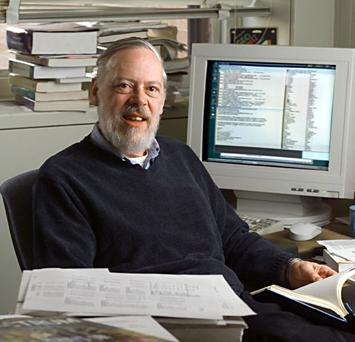
\includegraphics{gfx/dennis_ritchie6} \\ \smallskip
    Dedicado a la memoria de Dennis Ritchie \\ \smallskip
    1941\,--\,2011
\end{center}
%\cleardoublepage\include{FrontBackmatter/Foreword}
\cleardoublepage%*******************************************************
% Abstract
%*******************************************************
%\renewcommand{\abstractname}{Abstract}
\pdfbookmark[1]{Resumen}{Resumne}
\begingroup
\let\clearpage\relax
\let\cleardoublepage\relax
\let\cleardoublepage\relax

\chapter*{Resumen}
En los organismos sexuados, la fecundación es un proceso fundamental para la preservación de la vida. En este evento es necesario que el espermatozoide nade en busca del óvulo. Uno de los organismos modelo que se ha utilizado para estudiar este proceso es el erizo de mar, que produce una gran cantidad de espermatozoides en cada eyaculación y cuyo proceso de feundación es externo.

En este organismo modelo, varios resultados experimentales han relacionado distintos patrones de nado con una vía de señalización bioquímica que, al ser excitada por una molécula llamada speract que es liberada por el óvulo, induce un proceso de polarización y depolarización de la membrana celular del flagelo del espermatozoide. Este proceso de polarización y depolarización se debe a la entrada y salida de iones a través de distintos canales iónicos situados en la membrana. A través de un marcador fluorescente, es posible medir experimentalmente la concentración intracelular de uno de estos iones, el calcio.

En su estado nativo, el espermatozoide nada en modo circular. En la cercanía del óvulo, el espermatozoide se ve expuesto a un gradiente de speract, lo cual activa la vía de señalización antes mencionada. Como consecuencia de esta activación, el espermatozoide hace un giro brusco, seguido de un pequeño período en el que parece nadar de manera recta para luego intentar recuperar su nado circular. Cada molécula de speract que logra pegarse al receptor específico en la membrana del flagelo induce nuevamente esta vía, por lo cual se puede observar una alternancia de giros bruscos y nado recto. 

En una especie de erizo, este proceso parece ser guiado conforme el espermatozoide nada hacia el lugar donde la concentración de speract es mayor, es decir, en dirección hacia el óvulo. En este sentido se puede decir que el speract funciona como un quimioatractor para el espermatozoide. Sin embargo, en otra especie de erizo el espermatozoide presenta los giros bruscos causados por el speract, pero no parece ser atraído hacia el óvulo. Si bien diferentes resultados experimentales han sido de utilidad para establecer cuáles componentes bioquímicos toman parte en la vía de señalización y por ende de la maquinaria de control de motilidad del espermatozoide, aún quedan preguntas por responder con respecto al papel que juega cada uno de dichos componentes en la dinámica de la via de señalización. 

En este sistema biológico, probar diferentes estados y condiciones de manera experimental requiere de metodologías muy elaboradas. Sin embargo, también es posible utilizar distintas clases de modelos computacionales, con los cuales se simule una gran cantidad de condiciones y estados.

Se pueden crear distintos tipos de modelos dinámicos de acuerdo a diferentes criterios y formalismos, que van desde aquellos en los que no se considera el espacio, el tiempo y estado de los componentes del sistema son descritos de manera discreta; a aquellos en los que espacio, tiempo y estado son variables continuas. Así mismo, hay modelos que incorporan variables estocásticas para describir el comportamiento del sistema a través del tiempo. Cada formalismo requiere de una cantidad y calidad distinta de datos.

Entre los modelos que requieren una menor cantidad de datos se encuentran las redes lógicas, donde tiempo y estado son discretos, y cada componente del sistema actualiza su valor en el tiempo de acuerdo a una regla de evolución discreta. A pesar de su simplicidad, estos modelos han demostrado una gran capacidad de recuperar de manera cualitativa el comportamiento de un sistema, a la par que son capaces de generar predicciones nuevas que sugieran comportamientos susceptibles de ser verificados de manera experimental.

En particular, el artículo de \citet{Espinal2011} presenta un modelo discreto en tiempo y estado para la vía de señalización antes mencionada. Este modelo logró reproducir observaciones experimentales a la par de sugerir la existencia de comportamientos que no se habían estudiado anteriormente, y que fueron corroborados al realizar experimentos bajo las condiciones señaladas por la nueva predicción.

A pesar del éxito obtenido por este modelo, el tipo de comparaciones que pueden hacerse con las mediciones experimentales se mantiene a un nivel cualitativo. Para poder realizar comparaciones cuantitativas, se requiere que tiempo, estado o ambos sean variables continuas. Una manera de resolver este problema es construir un modelo consistente en un conjunto de ecuaciones diferenciales ordinarias \textsc{EDOs} que reproduzcan, al igual que el modelo discreto, las observaciones experimentales. Sin embargo, los modelos basados en \textsc{EDOs} requieren de un conocimiento más detallado de las interacciones, así como de las concentraciones de los distintos componentes de una vía de señalización. En particular para esta vía de señalización, muchas de estas cantidades no son conocidas, y medirlas experimentalmente es un proceso complicado y en muchas ocasiones costoso. 

Una alternativa es retomar el modelo discreto y transformarlo al formalismo de las ecuaciones de Glass. Este tipo de ecuaciones son de tipo diferencial lineal por pedazos, es decir, la dinámica del sistema se divide en intervalos de tiempo muy pequeños, y se definen sendas ecuaciones diferenciales lineales. La forma específica que toma la ecuación diferencial depende del valor de la función discreta sobre la cual se construyó dicha ecuación.

Las ecuaciones de Glass permiten hacer una comparación más directa con mediciones y condiciones experimentales. A pesar de que su formulación es muy sencilla, requieren de la estimación de un conjunto de parámetros, relacionados con el tiempo característico de reacción de cada componente y parámetros de umbral. Estos umbrales permiten discretizar mediante funciones escalón las variables de estado continuas, de modo que puedan ser evaluadas adecuadamente por las funciones discretas y pueda obtenerse una forma concreta de ecuación diferencial en cada intervalo de tiempo.

Elegir adecuadamente un conjunto de parámetros tales que reproduzcan las mediciones experimentales de calcio y concuerden con el conocimiento biológico de los distintos componentes de la vía de señalización, no es un problema trivial. Sin embargo, la estimación de parámetros puede ser expresada como un problema de optimización, en la que se busque minimizar la diferencia entre dos trayectorias a lo largo del tiempo.

El hecho de plantear un problema de optimización requiere del uso de estrategias de exploración del espacio de soluciones de la función objetivo, especialmente cuando no se tiene una idea clara de los gradientes de la función objetivo. Algunas estrategias de exploración incluyen búsqueda aleatoria, algoritmos genéticos y evolución diferencial. Estos dos últimos son estrategias evolutivas que han demostrado su utilidad en una gran variedad de situaciones para las cuales el paisaje de la función objetivo no es necesariamente diferenciable y en general para cuando este no es conocido ampliamente.

Como una primera aproximación al problema de transformar un sistema discreto en uno semicontinuo, se consideró un modelo de red Booleana de tres nodos que se transformó en un sistema de ecuaciones de Glass sincronizado. Una de las soluciones fue considerada como señal experimental y se puso en marcha la estimación de los parámetros que generaron dicha señal. En este caso se pudieron recuperar los parámetros que generaron dicha señal.

En el caso del modelo para la red de señalización, se usó la noción de distancia para comparar las mediciones experimentales de calcio con la dinámica de Glass del nodo que representa al calcio, y se presentan los resultados obtenidos.

Esta tesis se organiza como sigue: en el capítulo \ref{ch:antecedentes} se discute brevemente el fenómeno biológico que se quiere entender a través de modelación computacional. Posteriormente se discuten un modelo de red Booleana de tres nodos que se usó para ganar entendimiento de cómo transformar un modelo discreto en uno semicontinuo, así como del modelo de la vía de señalización basado en funciones discretas. El capítulo \ref{ch:matmet} presenta una discusión de los alcances y limitaciones del modelo discreto a manera de motivación y justificación para el desarrollo de este trabajo; posteriormente introduce el formalismo de ecuaciones de Glass; plantea el problema de la estimación de parámetros como un problema de optimización, describiendo las nociones de distancia usadas para comparar la dinámica de calcio de Glass con mediciones experimentales; finalmente aborda brevemente el procedimiento seguido para poner en marcha la búsqueda de parámetros.
\ref{ch:resultados} presenta los resultados de la búsqueda de parámetros. Posteriormente se presentan conclusiones y trabajo a futuro en \ref{ch:conclusiones}. Finalmente se presenta la bibliografía consultada para este proyecto.

\endgroup			

\vfill
%\cleardoublepage%*******************************************************
% Publications
%*******************************************************
\pdfbookmark[1]{Publications}{publications}
\chapter*{Publications}
Some ideas and figures have appeared previously in the following publications:

\bigskip

\noindent Put your publications from the thesis here. The packages \texttt{multibib} or \texttt{bibtopic} etc. can be used to handle multiple different bibliographies in your document.
\cleardoublepage%*******************************************************
% Acknowledgments
%*******************************************************
\pdfbookmark[1]{Acknowledgments}{acknowledgments}

\begin{flushright}{\slshape    
    [C has] the power of assembly language,\\
and the convenience of\dots assembly language.}\\
\medskip
    --- dmr, Dennis Ritchie.
\end{flushright}



\bigskip

\begingroup
\let\clearpage\relax
\let\cleardoublepage\relax
\let\cleardoublepage\relax
\chapter*{Agradecimientos}
Gracias a todos, yadda yadda.\\

\bigskip

Este trabajo cont\'o con una beca de maestr\'ia por parte de \textsc{conacyt} con n\'umero 241439.
Adem\'as, se cont\'o con el apoyo del proyecto \textsc{papiit in-109210} de la \textsc{dgapa-unam}.
\endgroup




\pagestyle{scrheadings}
\cleardoublepage%*******************************************************
% Table of Contents
%*******************************************************
%\phantomsection
\refstepcounter{dummy}
\pdfbookmark[1]{\contentsname}{tableofcontents}
\setcounter{tocdepth}{2} % <-- 2 includes up to subsections in the ToC
\setcounter{secnumdepth}{3} % <-- 3 numbers up to subsubsections
\manualmark
\markboth{\spacedlowsmallcaps{\contentsname}}{\spacedlowsmallcaps{\contentsname}}
\tableofcontents 
\automark[section]{chapter}
\renewcommand{\chaptermark}[1]{\markboth{\spacedlowsmallcaps{#1}}{\spacedlowsmallcaps{#1}}}
\renewcommand{\sectionmark}[1]{\markright{\thesection\enspace\spacedlowsmallcaps{#1}}}
%*******************************************************
% List of Figures and of the Tables
%*******************************************************
\clearpage

\begingroup 
    \let\clearpage\relax
    \let\cleardoublepage\relax
    \let\cleardoublepage\relax
    %*******************************************************
    % List of Figures
    %*******************************************************    
    %\phantomsection 
    \refstepcounter{dummy}
    %\addcontentsline{toc}{chapter}{\listfigurename}
    \pdfbookmark[1]{\listfigurename}{lof}
    \listoffigures

    \vspace*{8ex}

    %*******************************************************
    % List of Tables
    %*******************************************************
    %\phantomsection 
    \refstepcounter{dummy}
    %\addcontentsline{toc}{chapter}{\listtablename}
    \pdfbookmark[1]{\listtablename}{lot}
    \listoftables
        
    \vspace*{8ex}
%   \newpage
    
    %*******************************************************
    % List of Listings
    %*******************************************************      
	  %\phantomsection 
    \refstepcounter{dummy}
    %\addcontentsline{toc}{chapter}{\lstlistlistingname}
    \pdfbookmark[1]{\lstlistlistingname}{lol}
    \lstlistoflistings 

    %\vspace*{8ex}
       
    %*******************************************************
    % Acronyms
    %*******************************************************
    %\phantomsection 
    \refstepcounter{dummy}
    \pdfbookmark[1]{Acronyms}{acronyms}
    \markboth{\spacedlowsmallcaps{Acronyms}}{\spacedlowsmallcaps{Acronyms}}
    \chapter*{Abreviaturas}
    \begin{acronym}[hcn]
        \acro{ca}[$Ca^{2+}$]{calcio}
        %\acro{sp}[\emph{speract}]{speract}
        \acro{SR}[$SR$]{receptor de speract}
        \acro{gc}[$GC$]{guanilato ciclasa}
        \acro{GMP}[$GMP$]{guanosín monofosfato}
        \acro{cGMP}[$cGMP$]{guanosín monofosfato cíclico}
        \acro{pota}[$K^+$]{potasio}
        \acro{kcng}[$KCNG$]{canal de potasio regulado por cGMP}
        \acro{v}[$V$]{potencial de membrana}
        \acro{nce}[$NCE$]{intercambiador sodio–calcio}
        \acro{calintra}[\ensuremath{\left[Ca^{2+}\right]_i}]{calcio intracelular}
        \acro{nhe}[$NHE$]{intercambiador sodio–protones}
        \acro{phi}[$pH_i$]{pH intracelular} %$Na^+/Ca^{2+}$}
        \acro{hcn}[$HCN$]{canal activado por hiperpolarización y regulado por nucleótidos cíclicos}
        \acro{hva}[$HVA$]{canal de Calcio dependiente de alto voltaje}
        \acro{lva}[$LVA$]{canal de Calcio dependiente de bajo voltaje}
        \acro{AC}[$AC$]{adenilato ciclasa}
        \acro{cAMP}[$cAMP$]{Adenosín Monofosfato Cíclico}
        \acro{cAMPCC}[$cAMPCC$]{canal de calcio dependiente de cAMP}
        \acro{cacc}[$CaCC$]{canal de calcio dependiente de cloro}
        \acro{cakc}[$CaKC$]{canal de calcio dependiente de potasio}
        \acro{cap}[$CaP$]{bombas de calcio}
        \acro{dK}[$dK$]{permeabilidad de potasio}
        \acro{pde}[$PDE$]{fosfodiesterasa}
        \acro{EDOs}{ecuaciones diferenciales ordinarias}
    \end{acronym}                     
\endgroup

\cleardoublepage
%********************************************************************
% Mainmatter
%*******************************************************
\pagenumbering{arabic}
%\setcounter{page}{90}
% use \cleardoublepage here to avoid problems with pdfbookmark
\cleardoublepage
%\part{Some Kind of Manual}
%*****************************************
\chapter{Antecedentes}\label{ch:antecedentes}
%*****************************************

En este capítulo se discute brevemente el fenómeno biológico que se quiere entender a través de modelación computacional. Posteriormente se discuten un modelo de red Booleana de tres nodos que se usó para ganar entendimiento de cómo transformar un modelo discreto en uno semicontinuo, así como del modelo de la vía de señalización basado en funciones discretas. Este último modelo es un antecedente directo del semicontinuo desarrollado en este trabajo.

\section{Antecedentes biol\'ogicos}

La fertilización es un proceso crucial para la transmisión de la vida, que requiere el encuentro y fusión de los gametos. Para que este encuentro tenga lugar, el espermatozoide debe valerse de una intrincada maquinaria en su flagelo que le permita nadar en busca del óvulo. En algunas especies, el óvulo secreta una sustancia quimioatrayente que guía al esperma hacia él. En el caso particular del erizo de mar, esta sustancia es un decapéptido llamado \emph{speract}, el cual se une a un receptor específico en la membrana del flagelo del espermatozoide. La unión de speract con su receptor activa una red de señalización que produce oscilaciones en la concentración interna de algunos iones, de los cuales el principal es el calcio. 

La vía de señalización inducida por speract provoca la apertura de distintos canales que hiperpolarizan la membrana, es decir, que disminuyen drásticamente la polaridad de la membrana. A su vez, esta hiperpolarización cancela la desactivación de canales regulados por voltaje, que al abrirse despolarizan la membrana. La despolarización se refiere al proceso de regresar la polaridad de la membrana a sus niveles basales. El proceso repetido de hiper y despolarización se ha relacionado con cambios transitorios en la curvatura del flagelo del espermatozoide que resultan en modificaciones abruptas de su trayectoria. Estos cambios de trayectoria son una parte esencial para la motilidad y reorientación del esperma. De ahí la importancia de entender los mecanismos bioquímicos que la generan. 

Las oscilaciones de \textsc{calcio intracelular} $[Ca^{2+}]_i$ se caracterizan por presentar un incremento sostenido \emph{(tónico)} y fluctuaciones superimpuestas \emph{(supratónico)}, tal como se muestra en la figura \ref{fig:fluorescencia}. Se cuenta con mediciones experimentales de la vía de señalización que son obtenidas al añadir un marcador fluorescente al calcio. Al estimularse la vía mediante la adición de speract al medio, es posible observar dichos incrementos tónico y supratónico en la concentración de calcio. Los datos fueron obtenidos por Adán Guerrero en el laboratorio del Dr. Alberto Darszon. \citeauthor{Darszon2008} \citep{Darszon2008} y \citeauthor{Wood2007} \citep{Wood2007} presentan una descripción más detallada del tipo de técnicas experimentales usadas para la obtención de estos datos.
\\

\begin{figure}[hbt]
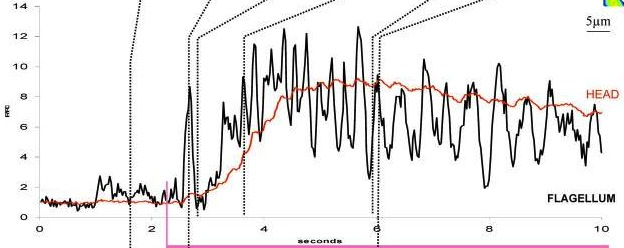
\includegraphics[width=0.9\linewidth]{gfx/maderaSperact}
\caption[Medición experimental de calcio intracelular]{Medición experimental de fluorescencia de calcio intracelular en espermatozoides. Las oscilaciones tónicas corresponden al incremento sostenido en la concentración de calcio, y tienen una forma sigmoidal. Este tipo de oscilaciones se presentan tanto en la cabeza como en el flagelo del espermatozoide. En la figura, la serie en rojo corresponde a la concentración de calcio en la cabeza, mientras que los datos en color negro corresponden a la concentración de calcio en el flagelo. Las oscilaciones supratónicas se observan solamente en el flagelo y se distinguen por ser las fluctuaciones que parecen "montarse"\ sobre la curva con forma sigmoidal. La barra de color rojo en la parte inferior, que inicia poco después de la marca de los 2 segundos muestra el momento en el que el speract comienza a estimular la vía de señalización y el tiempo en la que ésta se mantiene activa. Figura modificada tomada de \citeauthor{Wood2003} \citep{Wood2003}.}\label{fig:fluorescencia}
\end{figure}


Vistos a detalle, los eventos de la vía de señalización que se muestra en la figura \ref{fig:erizobBioquimica}, inician con la unión de speract a su \textsc{receptor} $(SR)$, que interacciona con una \textsc{Guanilato Ciclasa} $(GC)$ que produce \textsc{Guanosín Monofosfato(GMP) cíclico} $(cGMP)$. El aumento en la concentración de $cGMP$ abre el canal $(KCNG)$, que es un \textsc{canal de potasio} $(K^+)$ \textsc{regulado por cGMP}. La apertura de $(KCNG)$ resulta en la hiperpolarización del \textsc{potencial de membrana} $(V)$. Como consecuencia de la hiperpolarización suceden cuatro eventos importantes: \begin{enumerate}
\item se activa un \textsc{intercambiador} $Na^+/Ca^{2+}$ $(NCE)$ que disminuye los niveles de \textsc{calcio intracelular} $[Ca^{2+}]_i$
\item se activa un \textsc{intercambiador} $Na^+/H^+$ ($NHE)$ que incrementa el \textsc{pH intracelular} $(pH_i)$
\item se activa un \textsc{canal activado por hiperpolarización y regulado por nucleótidos cíclicos} $(HCN)$
\item finalmente, la sustracción de la inactivación del \textsc{canal de Calcio dependiente de alto voltaje} $(HVA)$ y el \textsc{canal de Calcio dependiente de bajo voltaje} $(LVA)$
\end{enumerate}

\begin{figure}[hbt]
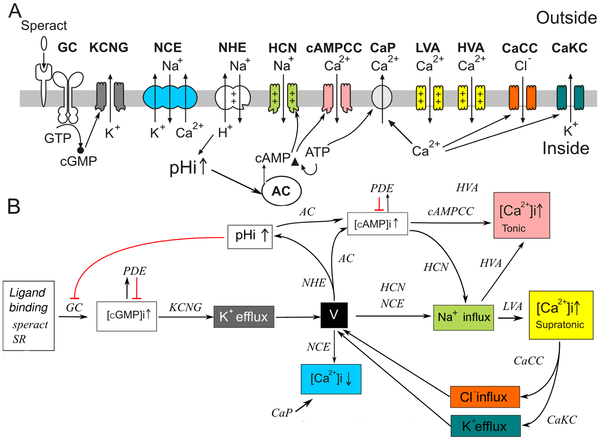
\includegraphics[width=0.9\linewidth]{gfx/redErizoBioquimica}
\caption[Red de se\~nalizaci\'on]{Red de se\~nalizaci\'on \citeauthor{Espinal2011} \citep{Espinal2011}.\ A) Componentes principales involucrados en la vía de señálización de speract. La unión de speract a su receptor en la membrana del flagelo dispara la cascada que produce cambios en $[Ca^{2+}]_i$ de dos maneras: un incremento sostenido (tónico) y fluctuaciones superimpuestas (supratónico). B) Eventos producidos por la vía de señalización.}\label{fig:erizobBioquimica}
\end{figure}

El incremento del $pH_i$ disminuye la actividad de $GC$ a la vez que activa una \textsc{adenilato ciclasa soluble} $(sAC)$, con la consecuente producción de \textsc{Adenosín Monofosfato Cíclico} $(cAMP)$. Este último estimula un \textsc{canal de calcio dependiente de cAMP} $(cAMPCC)$ y el canal $HCN$ previamente activado, lo cual tiende a repolarizar el potencial de membrana. Esta repolarización abre los canales $HVA$ y $LVA$ causando una despolarización y un incremento del $[Ca^{2+}]_i$. Finalmente, la vía de señalización se inicia de nuevo, posiblemente a través de un \textsc{canal de} $Ca^{2+}$ \textsc{dependiente de} $Cl^-$ $(CaCC)$ y un \textsc{canal de} $Ca^{2+}$ \textsc{dependiente de} $K^+$ $(CaKC)$, que se abren cuando la concentración de $[Ca^{2+}]_i$ es alta. Los mecanismos pasivos y constantes de extrusión de $Ca^{2+}$, tales como \textsc{bombas de calcio} $(CaP)$ y $NCE$, mantienen los niveles basales de $[Ca^{2+}]_i$. El mecanismo anteriormente descrito es repetido cíclicamente, generando un tren de oscilaciones de $Ca^{2+}$ que produce una secuencia repetitiva de cambios de dirección en el espermatozoide. En un experimento típico, como el mostrado en la figura \ref{fig:fluorescencia}, la vía se mantiene activa un promedio de 10 segundos \citeauthor{Wood2003} \citep{Wood2003}.

\section{Antecedentes de modelos discretos}

Los modelos de red Boolena (o más generalmente, modelos discretos) son discretos en tiempo y estado, donde cada componente de una vía de señalización  bioquímica o red regulatoria genética se considera como un nodo. La red está formada por estos nodos y un conjunto de aristas, que representan el tipo de interacción existente entre cada par de nodos. Estas interacciones pueden ser de activación o de inhibición. 

En cada paso de tiempo $t$ un nodo de la red puede encontrarse en un estado $0$ ó $1$. El $0$ representa actividad basal o inactividad, mientras que el $1$ representa actividad o expresión. En general, se pueden establecer distintos niveles de expresión o actividad si se considera que los nodos puedan tomar valores discretos, i.e. $0, 1, -1, 2,$ etc.

El sistema evoluciona a través del tiempo mediante una regla de evolución. Cada nodo $i$ de la red tiene asociada una de estas reglas de evolución,  que depende de $k$ nodos reguladores de $i$, es decir, aquellos nodos que tienen una arista incidente en el nodo $i$. Si denotamos el estado del nodo $i$ en el tiempo $t$ con $\sigma_i(t)$, tenemos el mapeo discreto

\begin{equation}\label{eqn:kaufman}
\sigma_i(t+1) = F_i[\sigma_{i_1}(t), \sigma_{i_2}(t),\ldots, \sigma_{i_k}(t)]
\end{equation}

Iterando esta regla de evolución para cada nodo de la red se obtiene una descripción por pulsos de la dinámica del sistema. Cada pulso puede ser considerado como el promedio discretizado de la variable de estado de cada nodo de la red durante un intervalo de tiempo dado. Si bien el $(t+1)$ en la función de evolución se refiere a un tiempo de máquina o tiempo de simulación, es posible hacer comparaciones entre este tiempo de máquina y el tiempo de los experimentos.

Uno de los aspectos fundamentales de este tipo de modelos discretos es que cualquier configuración inicial posible de estados del sistema llega a un conjunto de configuraciones que se repiten a lo largo del tiempo tras iterar un cierto número de veces la reglas de evolución de la red. Estas configuraciones repetidas pueden ser puntuales, es decir, la misma configuración se repite \emph{ad eternum}; o bien cíclicas, es decir, el sistema vuelve a la misma configuración después de un cierto número de pasos de tiempo. En ambos casos, el conjunto de los estados que se repiten una y otra vez, se conoce como atractor. El conjunto de todas las configuraciones iniciales que tras iterar la regla de evolución del sistema alcanzan un atractor, se conoce como cuenca de atracción. Las configuraciones que se encuentran entre una condición inicial y un atractor, se conocen como transitorios.

\citeauthor{huang2005} \citep{huang2005} muestran que los atractores din\'amicos corresponden a patrones estables de expresi\'on gen\'etica que determinan estados funcionales estables de una c\'elula. En el caso del modelo de la red de se\~nalizaci\'on que se estudia en este trabajo, los atractores de la red determinan las oscilaciones estables de calcio que posibilitan la relocalizaci\'on de los espermatozoides a trav\'es de las alteraciones que el calcio induce a la curvatura del flagelo.

\subsection{Modelo discreto de tres nodos}\label{sect:3nodos}

%% ESTA SUBSECCIóN REQUIERE UN MAJOR REWRITING :S

Con el objetivo de explorar y ganar entendimiento acerca de cómo transformar modelos discretos en modelos de Glass, se utilizó una red Booleana de tres nodos que había sido estudiada previamente por \citeauthor{Reka3Nodos2010}. En ese trabajo se caracteriza por completo el comportamiento de dicha red discreta. Este modelo discreto es mostrado en la figura \ref{fig:red3reka}.

\begin{figure}[hbt]
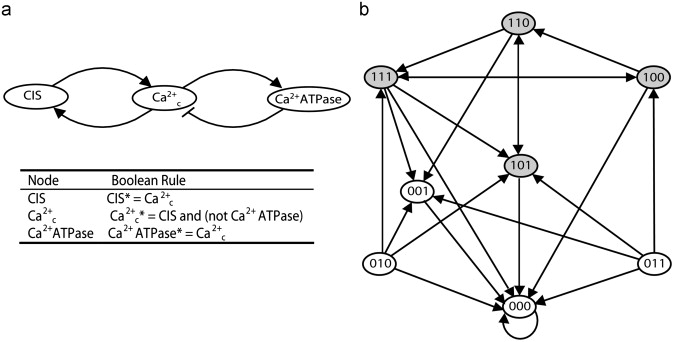
\includegraphics[width=0.9\linewidth]{gfx/red3nodos}
\caption[Modelo Booleano de 3 nodos]{Modelo Booleano de 3 nodos de \citeauthor{Reka3Nodos2010} \citep{Reka3Nodos2010}.\ a) Reglas L\'ogicas.\ b) Estados posibles de la red.}\label{fig:red3reka}
\end{figure}


Si bien este modelo no está relacionado con la red de señalización discutida en esta tesis, el hecho de contar con pocos nodos sirvió como un buen punto de partida para transformar un modelo Booleano en uno de ecuaciones de Glass.

\subsection{Modelo discreto de la vía de señalización inducida por speract}\label{sect:erizo}


\citeauthor{Espinal2011} \citep{Espinal2011} presentan un modelo discreto en tiempo y estado para la vía de señalización inducida por speract en el flagelo del esperma de erizo de mar. En ese trabajo, dieciocho de los veintidos nodos toman valores de estado $0$ ó $1$, mientras que los cuatro nodos restantes tienen un valor de estado ternario, es decir, cada uno de estos nodos puede encontrarse en el estado $0$, $1$ ó $2$. Esta extensión a tres valores posibles es necesaria para capturar los estados posibles en los que se puede encontrar un componente de la red, véase la figura \ref{fig:erizoModelo}.

\begin{figure}[hbt]
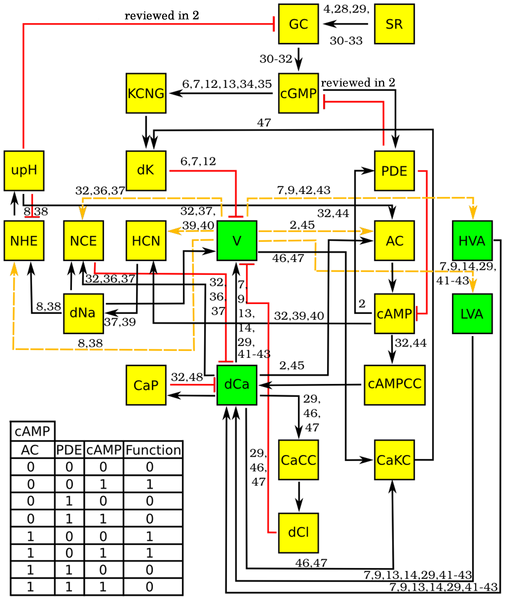
\includegraphics[width=0.9\linewidth,height=10cm]{gfx/redErizoModelo}
\caption[Modelo Discreto de la red de se\~nalizaci\'on]{Modelo Discreto de la red de se\~nalizaci\'on \citeauthor{Espinal2011} \citep{Espinal2011}.\ Los cuadros amarillos y verdes indican nodos binarios y ternarios, respectivamente. Las flechas negras indican activación, las líneas rojas inhibición y las flechas amarillas pueden representar activación o inhibición, dependiendo del valor del nodo de voltaje $(V)$. Los números sobre las flechas corresponden a las referencias con las que \citeauthor{Espinal2011} \citep{Espinal2011} construyeron la red y sustentan cada interacción. A manera de ejemplo, la función reguladora o tabla de verdad del nodo de $cAMP$ se muestra en la esquina inferior izquierda. Las primeras 3 columnas en esta tabla contienen todos los valores posibles de activación de los reguladores de $cAMP$, $(AC,\ PDE,\ cAMP)$; la cuarta columna muestra los valores para la función que corresponden a cada combinación de los reguladores.}\label{fig:erizoModelo}
\end{figure}


\begin{figure}[hbt]
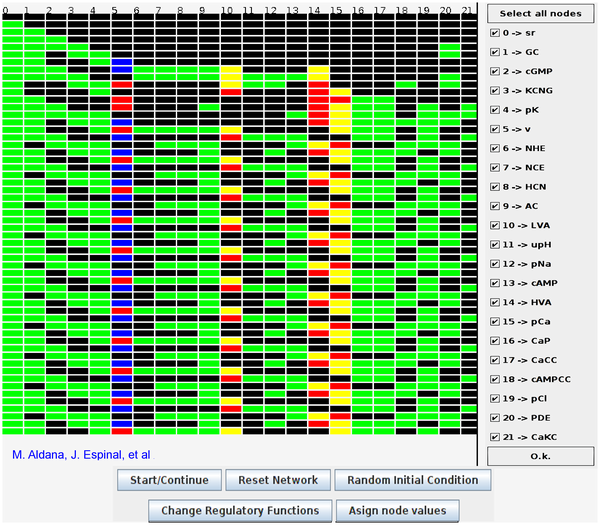
\includegraphics[width=0.9\linewidth%,height=10cm
]{gfx/appletErizo}
\caption[Applet del Modelo Discreto]{Applet del Modelo Discreto de la red de se\~nalizaci\'on \citeauthor{Espinal2011} \citep{Espinal2011}.\ Serie temporal de los patrones de activación de la red de señalización bajo diferentes condiciones. En cada caso, los nodos están en el eje horizontal y el tiempo en el eje vertical. Para los nodos binarios, el negro representa el estado \emph{apagado}, verde \emph{encendido}. Los nodos $10$ y $14$, correspondientes al $HVA$ y $LVA$, el negro es un estado inactivo, el amarillo corresponde a un canal cerrado y el rojo a un canal abierto. El nodo 5, correspondiente al potencial de membrana $V$ es negro para un potencial en reposo, azul para la hiperpolarización y rojo para la repolarización. El nodo 15 $(dCa)$, correspondiente al $Ca^{2+}$ es amarillo para indicar el incremento tónico, rojo para el incremento supratónico y negro para indicar estado basal. Como puede observarse, tras un transitorio la red llega a un atractor de período 4. Se muestra el comportamiento del especímen silvestre (wt).
El applet fue desarrollado por el Dr. Maximino Aldana y se encuentra disponible en \url{http://www.fis.unam.mx/research/seaurchin/discrete/}. Este applet permite explorar de manera interactiva distintas condiciones iniciales, cambiar las reglas lógicas así como observar el comportamiento de la red en ausencia de algunos nodos.}\label{fig:appletErizo}
\end{figure}

En el trabajo citado, se determina que este modelo llega a dos configuraciones cíclicas o atractores, uno de período cuatro y otro de período ocho. Estos atractores se relacionaron con las mediciones experimentales de fluorescencia de calcio en el flagelo del espermatozoide. El 80\% de las configuraciones iniciales posibles convergen al atractor de período cuatro. El período cuatro de este atractor corresponde a una oscilación del tren de oscilaciones que se observa en las mediciones experimentales como la de la figura \ref{fig:fluorescencia} \citeauthor{Espinal2011} \citep{Espinal2011}.

Un paso fundamental al proponer un modelo para un sistema biológico consiste en comparar los resultados de dicho modelo con comportamientos que se hayan observado previamente mediante técnicas experimentales. A este proceso se le conoce como validación del modelo. El modelo presentado en \citeauthor{Espinal2011} \citep{Espinal2011} corrobora en un nivel cualitativo comportamientos observados experimentalmente, por ejemplo:
\begin{itemize}
\item En ausencia de speract, todas las condiciones iniciales alcanzan las condiciones basales tras un pequeño transitorio. De esta manera se confirma el papel que juega el speract para disparar las oscilaciones de $[Ca^{2+}]_i$.
\item Si el nodo correspondiente a la permeabilidad de potasio $(dK)$ se elimina, las oscilaciones de $[Ca^{2+}]_i$ se suprimen. Este comportamiento se ha observado experimentalmente en \citeauthor{Babcock:1992uf} \citep{Babcock:1992uf}.
\end{itemize}

Una de las ventajas de construir modelos dinámicos de vías de señalización es facilitar la simulación de una gran cantidad de condiciones experimentales, con la intención de realizar predicciones que sugieran experimentos nuevos.

\begin{figure}[hbt]
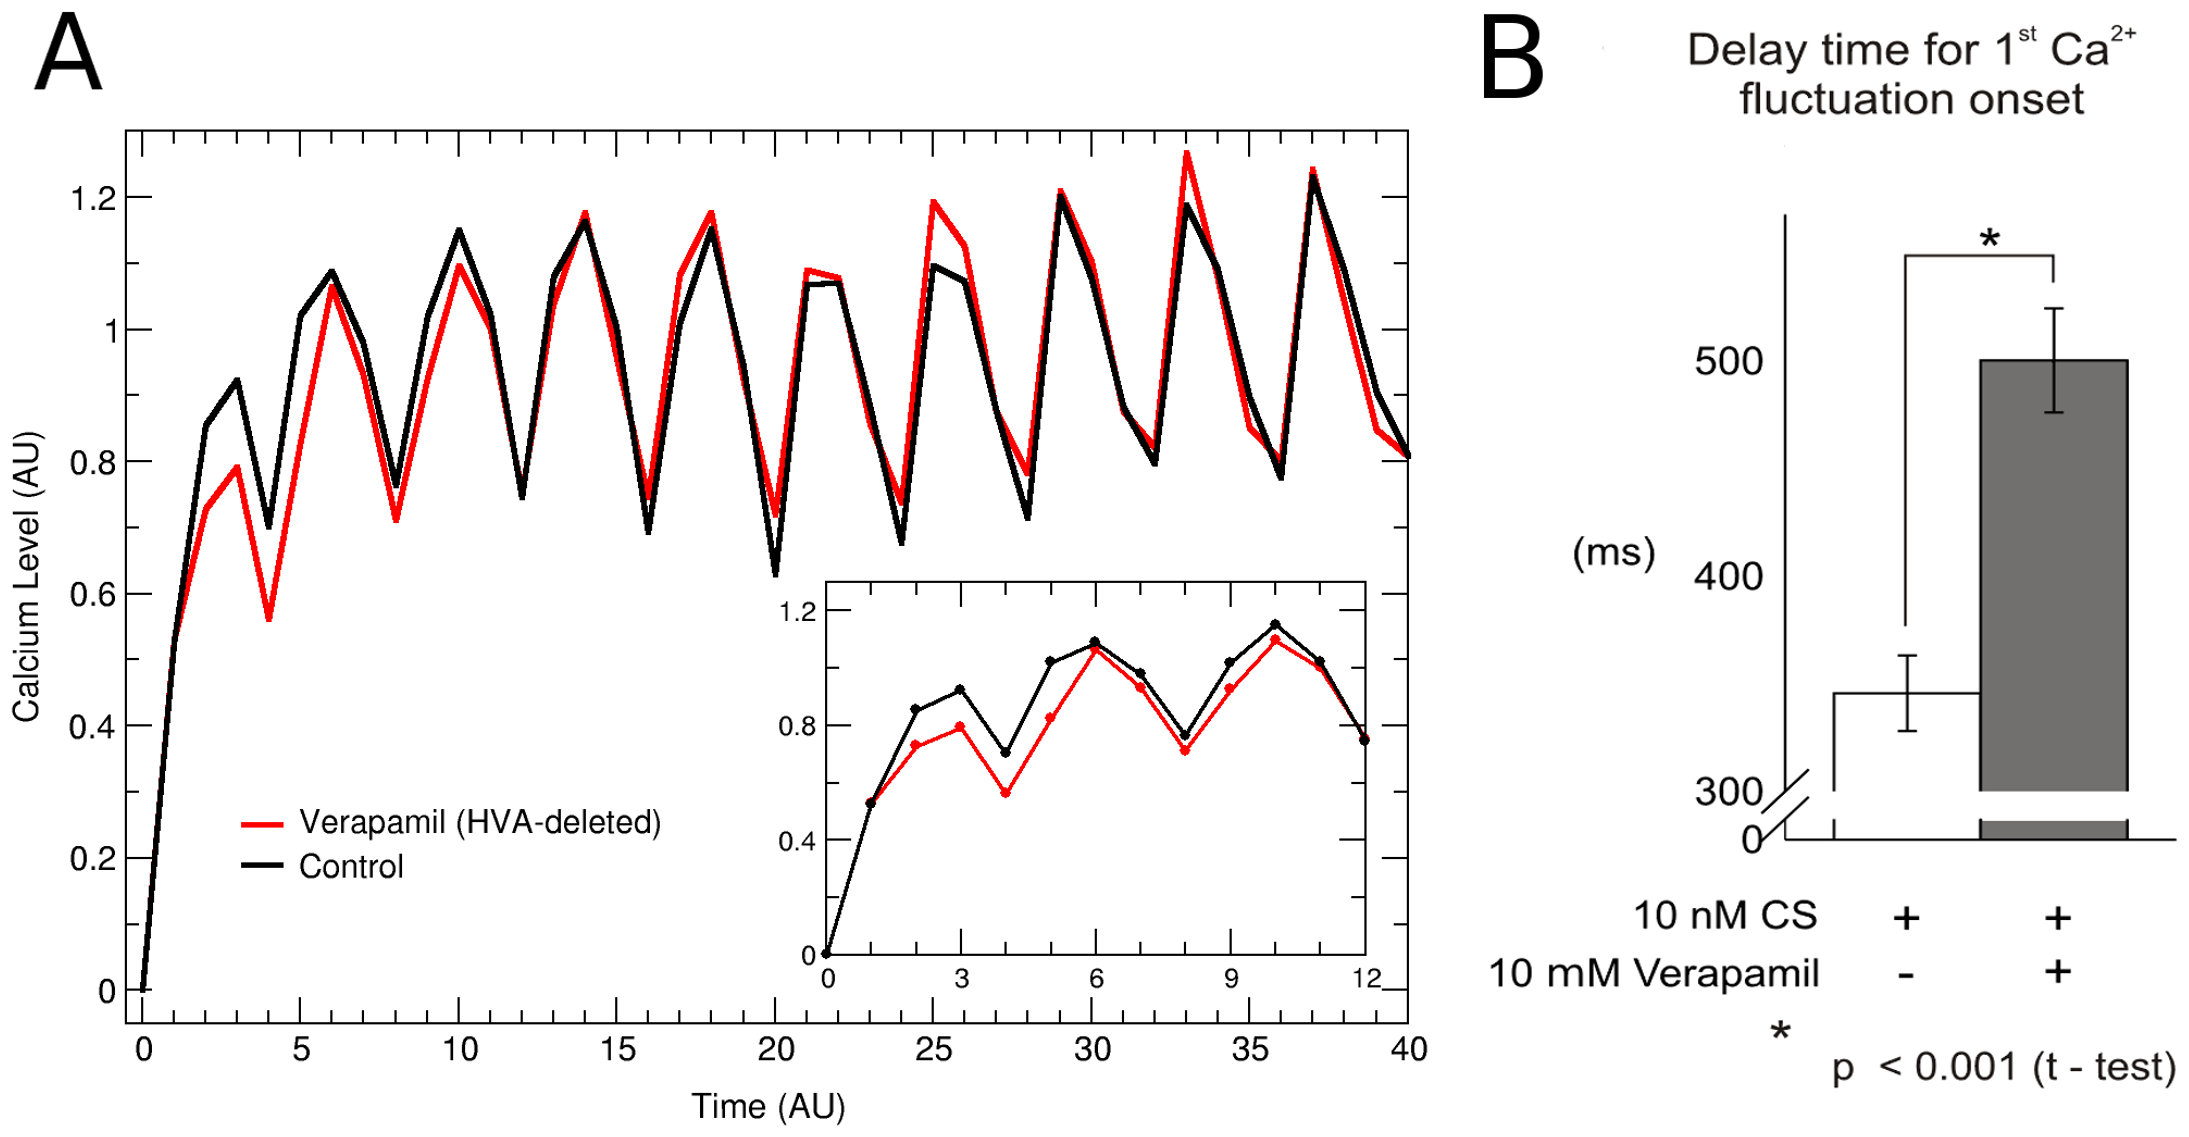
\includegraphics[width=0.9\linewidth]{gfx/figura8Chucho}
\caption[El bloqueo del canal HVA retrasa el inicio de las oscilaciones de calcio]{El bloqueo del canal HVA retrasa el inicio de las oscilaciones de calcio. A) Evolución temporal del nivel promedio de calcio tomado a cada paso de tiempo durante $10^5$ condiciones iniciales con $HVA$ (curva negra) y sin $HVA$ (curva roja), usando unidades arbitrarias. Nótese que cuando el canal $HVA$ está presente el incremento en los niveles de calcio comienza más rápidamente que cuando se suprime el canal $HVA$, es decir, en los primeros pasos de tiempo, la curva negra se incrementa antes que la curva roja. B) Los experimentos realizados muestran que el verapamil, sustancia que inhibe al canal $HVA$, prolonga el tiempo entre la estimulación de speract y el establecimiento de la primera fluctuación de calcio. \citeauthor{Espinal2011} \citep{Espinal2011}.}\label{fig:verapamil}
\end{figure}

El modelo de la vía de señalización de speract predijo dos comportamientos que no se habían observado experimentalmente. En particular, uno de ellos consiste en que al suprimir el canal $HVA$, aumenta el tiempo para que la concentración de calcio alcance los valores de alta intensidad que provoca la unión del speract a su receptor. Esta condición fue el comportamiento observado en promedio para $10^5$ condiciones iniciales diferentes. A raíz de este resultado del modelo se realizaron experimentos añadiendo $10  nm$ de \emph{verapamil}, un inhibidor del canal $HVA$. El bloqueo de este canal produce un retraso en la aparición de la primera fluctuación de $[Ca^{2+}]_i$ en el flagelo del espermatozoide, lo cual valida a un nivel cualitativo la predicción hecha por el modelo. Este resultado se muestra en la figura \ref{fig:verapamil}

Como se puede observar en el apartado B de la figura \ref{fig:verapamil}, el tiempo medio para la aparición de la primera oscilación de calcio tras la adición de speract al medio es de alrededor de $500 ms$ en presencia de verapamil, en contraste con los $~350 ms$ del tipo silvestre. 


%% Este párrafo quedaría mejor en la justificación del modelo semicontinuo.
Por lo tanto, el modelo discreto divide una oscilación de calcio en cuatro subintervalos discretos en el tiempo. El valor discreto de un nodo cualquiera de la red en un  subintervalo de tiempo, puede interpretarse como el promedio de los valores continuos que tomó ese nodo en el subintervalo: si dicho valor promedio fue mayor que un umbral, el estado discreto en todo el subintervalo es 1, y 0 en caso contrario. Lo que se quiere poner de manifiesto con esta observación es que las comparaciones entre un modelo discreto y las mediciones experimentales son a un nivel cualitativo y con una resolución temporal lo suficientemente grande como para contener en un paso de tiempo discreto varios cambios de estado continuo. Un modelo discreto es capaz de decir cómo cambia un sistema en una escala de tiempo más grande que aquella en la que suceden los eventos microscópicos del sistema. De ahí la necesidad de contar con otro tipo de descripciones del sistema que permitan hacer comparaciones entre modelo y experimentos en escalas de tiempo más pequeñas. Además, es deseable que dichas descripciones permitan hacer una comparación más precisa entre los valores de las variables de estado y las mediciones experimentales, por ejemplo, donde las variables de estado del modelo sean continuas.

%%(Insertar figura que explique esto).
%%Discusión aquí de algunos de los resultados del modelo discreto.

%\cleardoublepage
%\ctparttext{You can put some informational part preamble text here. 
%Illo principalmente su nos. Non message \emph{occidental} angloromanic
%da. Debitas effortio simplificate sia se, auxiliar summarios da que,
%se avantiate publicationes via. Pan in terra summarios, capital
%interlingua se que. Al via multo esser specimen, campo responder que
%da. Le usate medical addresses pro, europa origine sanctificate nos se.}
%\part{The Showcase}
%************************************************
\chapter{Materiales y M\'etodos}\label{ch:matmet} % $\mathbb{ZNR}$
%************************************************
%Este capítulo comienza con una discusión de los alcances y limitaciones del modelo discreto a manera de motivación y justificación para el desarrollo de este trabajo. Posteriormente introduce el formalismo de ecuaciones de Glass; plantea el problema de la estimación de parámetros como un problema de optimización, describiendo las nociones de distancia usadas para comparar la dinámica de calcio de Glass con mediciones experimentales; finalmente aborda brevemente el procedimiento seguido para poner en marcha la búsqueda de parámetros.

\section{Scratchpad}
En el caso de la vía de señalización, objeto de estudio de esta tesis, los parámetros a encontrar fueron aquellos tales que reprodujeran el comportamiento del calcio intracelular observado experimentalmente. Se tomó en consideración solamente la similitud en la dinámica de calcio del sistema debido a que éste es el único tipo de dato experimental que cuenta con mediciones largas. Un ejemplo de estas mediciones se muestra en la figura \ref{fig:fluorescencia}.


\subsection{Funciones objetivo}

Es necesario establecer una noción de distancia para determinar si la serie temporal proveniente de los experimentos de fluorescencia de calcio corresponde con la trayectoria del nodo de calcio del modelo de ecuaciones semicontinuas.

%
%\subsubsection{Sparsity Promoting Regularization}
%
%Una alternativa a otro tipo de comparaciones es la \textsc{Regularización Promotora de Dispersión o Sparsity Promoting Regularization}, \citeauthor{Engl2009}. La idea consiste en imputar un modelo estadístico a la comparación de mediciones experimentales con modelos de ecuaciones diferenciales. Los operadores diferenciales que no incluyen componentes estocásticos suelen producir trayectorias por lo general suaves, en contraste con la variabilidad existente en las series de tiempo de las mediciones experimentales. 
%
%Sea $\mathbf{p}$ el vector de parámetros de un conjunto de ecuaciones diferenciales. Sea $\Phi(\mathbf{p},t)$ la trayectoria solución dependiente del tiempo $t$ y del vector de parámetros $\mathbf{p}$. Sea $\Psi(\Phi(\mathbf{p},t))$ un modelo Gaussiano del ruido de las mediciones experimentales con desviación estándar constante. El objetivo de añadir $\Phi$  es imputar un criterio estadístico a la trayectoria solución de la ecuación diferencial, y hacer entonces una comparación entre un modelo estadísticos y un conjunto de datos.
%
%Bajo este esquema, se puede buscar minimizar
%\begin{equation}
%J(\mathbf{p}) = \| \Psi(\Phi(\mathbf{p},t)) - X\|_2^2 -\beta \| \mathbf{p} \| _1^1
%\end{equation}
%donde $\beta \in (0,1)$ es un término promotor de la regularización, que se utiliza para ponderar mediante la norma a 1 el desempeño del vector de parámetros $\mathbf{p}$, mientras que $X$ representa los datos contra los cuales se compara el modelo. 

En este trabajo, las estrategias de exploración utilizadas fueron \textsc{Búsqueda Aleatoria}, \textsc{Algoritmos Genéticos} y \textsc{Evolución Diferencial}, cada uno de los cuales se describe a continuación.

\subsubsection{Búsqueda Aleatoria}

La búsqueda aleatoria es la más simple de las estrategias de búsqueda. Consiste en elegir al azar una solución, evaluarla y, si y solo si su costo es mejor que el mejor costo hasta el momento, guardar la solución como la mejor hasta el momento; en caso contrario no se guarda la solución ni se actualiza el valor del mejor costo. En ambos casos, si no se ha llegado a una precisión determinada para la función de costo o bien se ha alcanzado un número máximo de iteraciones, la búsqueda finaliza; en caso contrario, se elige otra solución al azar y se repite el proceso.

\subsubsection{Algoritmos Genéticos}

Inspirados en el trabajo de \citeauthor{holland1975} \citep{holland1975} y tratados de manera un poco más rigurosa por \citeauthor{Goldberg1989} \citep{Goldberg1989}, los algoritmos genéticos son una estrategia de búsqueda que simula el proceso de evolución natural a través de los procesos de cruza, mutación y selección.

El agoritmo inicia con un conjunto de agentes denominados población, donde cada agente tiene un \emph{genoma}, es decir, una representación codificada de una solución al problema de optimización. Posteriormente se selecciona a algunos individuos de la población para procrear a la siguiente generación. La selección se realiza mediante diferentes esquemas, aunque en términos generales se suele favorecer a aquellos individuos que tengan un mejor costo. Los individuos no seleccionados no sobreviven. De entre aquellos que sí han sido seleccionados, se eligen pares de agentes y estos combinan su genoma de acuerdo a algún esquema para crear un tercer agente. Este proceso de cruza se realiza hasta completar una cantidad preestablecida de miembros de la nueva generación. Con cierta probabilidad, por lo general baja, algunos individuos de la nueva población sufrirán una mutación en su genoma. El proceso de selección, cruza y mutación continúa hasta que se ha alcanzado cierta precisión en el costo de la solución o bien se ha alcanzado un número determinado de iteraciones.

Tradicionalmente el genoma y los operadores de los algoritmos genéticos son discretos. Dado que los parámetros que se requirió estimar en este trabajo toman valores continuos, se usó una variante de los algoritmos genéticos tradicionales, adaptados a trabajar con variables continuas encontrado en \citeauthor{Haupt1998} \citep{Haupt1998}, en donde el genoma de un agente se codifica como un vector de valores continuos y los operadores de cruza y mutación pueden ser aplicados a este tipo de variables.

\subsubsection{Evolución Diferencial}

\citeauthor{Storn1997} \citep{Storn1997} observaron que algunos métodos heurísticos existentes no eran tan robustos y no convergían tan rápidamente al ser aplicados a problemas de optimización que involucraran variables continuas. A raíz de esto, desarrollaron un método específicamente pensado para este tipo de problemas. 

El método consiste en una población de soluciones candidato, llamadas agentes. Cada agente se mueve a través del espacio de búsqueda combinando las posiciones de los agentes existentes en la población. Si la nueva posición del agente representa una mejora, esta nueva posición se acepta y pasa a formar parte de la población; en caso contrario, la nueva posición se rechaza. El proceso se repite y se espera que una solución satisfactoria se descubrirá eventualmente.

Sea $x \in \mathbb{R}^n$ un agente en la población de tamaño $NP>3$; sea $F \in [0,2]$, conocido como peso diferencial; sea también $CR \in [0,1]$, la probabilidad de cruza. El algoritmo de evolución diferencial consiste en:
\begin{enumerate}
\item Inicializar cada agente $x$ con una posición aleatoria en el espacio de búsqueda.
\item Hasta que un criterio de búsqueda sea satisfecho, repetir:
	\begin{enumerate}
		\item Escoger al azar tres agentes distintos entre sí $a$, $b$, $c$.
		\item Escoger un índice al azar $R \in {1,\ldots,n}$ donde $n$ es la dimensionalidad del problema
		\item Calcular la posible nueva posición del agente, dada por $y=[y_1,\ldots,y_n]$ iterando sobre cada $i \in {1,\ldots,n}$ como sigue:
			\begin{enumerate}
				\item Elegir al azar de manera uniforme $r \in (0,1)$
				\item Si $i=R$ o $r_i<CR$, hacer $y_i=a_i+F(b_i-c_i)$. En caso contrario $y_i=x_i$
			\end{enumerate}
		\item Si $f(y)<f(x)$, entonces $x=y$
	\end{enumerate}
\item Elegir el agente con el menor costo o máxima adaptación y regresarlo como la mejor solución candidato encontrada.
\end{enumerate}

La elección de $F$, $CR$ y $NP$ puede tener un impacto significativo en el desempeño de la optimización. \citeauthor{Storn1997}  \citep{Storn1997}, y \citeauthor{lampinen2002} \citep{lampinen2002} proporcionan valores iniciales para estos parámetros que parecen ser un buen punto de partida en general.

\section{Búsqueda de parámetros}

La búsqueda de parámetros para los modelos de ecuaciones de Glass se realizó usando diferentes combinaciones de funciones objetivo y estrategias de búsqueda. La implementación de las rutinas se realizó en lenguaje C \citeauthor{Kernighan1988} \citep{Kernighan1988} bajo el estándar \textsc{iso c99} publicado por  \citeauthor{c99} \citep{c99} usando el compilador \textsc{clang} de \citeauthor{clang} \citep{clang}. Adicionalmente, se usaron los módulos de estadística, métodos de solución de ecuaciones diferenciales ordinarias, vectores y matrices, y generación de números aleatorios de la biblioteca de funciones para cómputo científico \textsc{GNU Scientific Library (GSL) v.1.15} \citeauthor{gslManual} \citep{gslManual}.

Para la solución de ecuaciones diferenciales se utilizó el método de Euler \citeauthor{numrecipesc} \citep{numrecipesc}. También se utilizaron el método de Runge-Kutta 4,5 \citeauthor{numrecipesc} \citep{numrecipesc}, \citeauthor{gslManual} \citep{gslManual}; y el método de paso adaptativo de Adams-Bashforth \citep{gslManual}. Estos dos últimos métodos son menos sensibles a errores que el método de Euler original.

El método de Euler se implementó directamente, mientras que para el caso del método de Runge-Kutta 4,5 y del método de Adams-Bashforth se utilizó la implementación de la \textsc{GNU Scientific Library (GSL) v.1.15}. La generación de números aleatorios se realizó usando la implementación de la \textsc{GNU Scientific Library (GSL) v.1.15} del algoritmo \textsc{ranlxs2} \citeauthor{gslManual} \citep{gslManual}.

Como esquema general, los programas de inferencia de parámetros consistían en proponer soluciones candidato y evaluarlas, repitiendo el proceso hasta cumplir con un criterio de paro. Una solución candidato consiste en un conjunto de parámetros propuestos de acuerdo a una estrategia de exploración del espacio de búsqueda y las trayectorias solución del problema de condiciones iniciales del sistema de ecuaciones de Glass correspondiente a dichos parámetros. La evaluación de candidatos consistió en comparar la señal original o medición experimental con la dinámica de Glass del nodo correspondiente a dicha señal o medición experimental.



%\addtocontents{toc}{\protect\clearpage} % <--- just debug stuff, ignore
%************************************************
\chapter{Resultados}\label{ch:resultados}
%************************************************
\section{Búsqueda de parámetros}

La búsqueda de parámetros para los modelos de ecuaciones de Glass se realizó usando diferentes combinaciones de funciones objetivo y estrategias de búsqueda. La implementación de las rutinas se realizó en lenguaje C \citep{Kernighan1988} bajo el estándar \textsc{iso c99} publicado por \citet{c99} usando el compilador \textsc{clang} \citep{clang}. Adicionalmente, se usaron los módulos de estadística, métodos de solución de ecuaciones diferenciales ordinarias, vectores y matrices, y generación de números aleatorios de la biblioteca de funciones para cómputo científico \textsc{GNU Scientific Library (GSL) v.1.15} \citep{gslManual}.

Para la solución de ecuaciones diferenciales se utilizó el método de Euler \citeauthor{numrecipesc} \citep{numrecipesc}. También se utilizaron el método de Runge-Kutta 4,5 \citeauthor{numrecipesc} \citep{numrecipesc}, \citep{gslManual}; y el método de paso adaptativo de Adams-Bashforth \citep{gslManual}. Estos dos últimos métodos son menos sensibles a errores que el método de Euler original.

El método de Euler se implementó directamente, mientras que para el caso del método de Runge-Kutta 4,5 y del método de Adams-Bashforth se utilizó la implementación de la \textsc{GNU Scientific Library (GSL) v.1.15}. La generación de números aleatorios se realizó usando la implementación de la \textsc{GNU Scientific Library (GSL) v.1.15} del algoritmo \textsc{ranlxs2}.

Como esquema general, los programas de inferencia de parámetros consistían en proponer soluciones candidato y evaluarlas, repitiendo el proceso hasta cumplir con un criterio de paro. Una solución candidato consiste en un conjunto de parámetros propuestos de acuerdo a una estrategia de exploración del espacio de búsqueda y las trayectorias solución del problema de condiciones iniciales del sistema de ecuaciones de Glass correspondiente a dichos parámetros. La evaluación de candidatos consistió en comparar la señal original o medición experimental con la dinámica de Glass del nodo correspondiente a dicha señal o medición experimental.

\subsection{Modelo de tres nodos}

Para el modelo discreto de tres nodos, dado por:

\begin{equation}
CIS(t+\tau) = Ca^{2+}(t)
\end{equation}

\begin{equation}
Ca^{2+}(t+\tau) = CIS(t) * (Ca^{2+}ATPase(t) + 1) \% 2)
\end{equation}

\begin{equation}
Ca^{2+}ATPase(t+\tau) = Ca^{2+}(t)
\end{equation} 
\\
se implementó un modelo semicontinuo con las siguientes ecuaciones de Glass:
\begin{equation}
\frac{dCIS}{dt} = \alpha_{CIS} [F_{CIS}(\widehat{Ca^{2+}}) - CIS]
\end{equation}

\begin{equation}
\frac{dCa^{2+}}{dt} = \alpha_{Ca^{2+}} [F_{Ca^{2+}}(\widehat{CIS}, \widehat{Ca^{2+}ATPase}) - Ca^{2+}]
\end{equation}

\begin{equation}
\frac{dCa^{2+}ATPase}{dt} = \alpha_{Ca^{2+}ATPase} [F_{Ca^{2+}ATPase}(\widehat{Ca^{2+}}) - Ca^{2+}ATPase)]
\end{equation} 
\\
donde
$$\widehat{CIS} = H(CIS - \theta_{CIS})$$
\\
$$\widehat{Ca^{2+}} = H(Ca^{2+} - \theta_{Ca^{2+}})$$
\\
$$\widehat{Ca^{2+}ATPase} = H(Ca^{2+}ATPase - \theta_{Ca^{2+}ATPase})$$
\\
corresponden a los valores discretizados de las variables continuas $CIS$, $Ca^{2+}$ y $Ca^{2+}ATPase$, respectivamente. Es necesario discretizar el valor de estas variables pues hay que recordar que $F_{CIS}$, $F_{Ca^{2+}}$ y $F_{Ca^{2+}ATPase}$ son funciones cuyos argumentos son valores discretos.

Como caso de ejemplo de estimación de parámetros en un problema de transformación de un modelo discreto a un modelo semicontinuo, se resolvió mediante el método de Euler el sistema de ecuaciones de Glass de la red de 3 nodos con parámetros $\alpha_{CIS} = \alpha_{Ca^{2+}} =  \alpha_{Ca^{2+}ATPase} = 1$, umbrales de activación $\theta_{CIS} = 0.3$, $\theta_{Ca^{2+}} = 0.7$ y $\theta_{Ca^{2+}APTase} = 0.8$, y $CIS = 1$, $Ca^{2+} = 0$, $Ca^{2+}ATPase = 0$ como condiciones iniciales. El objetivo consistió en encontrar mediante un procedimiento de búsqueda el conjunto de parámetros tales que la dinámica de Glass correspondiente al $Ca^{2+}ATPase$ fuera lo más similar posible a la solución conocida para los parámetros antes mencionados. Esta solución conocida se tomó como una señal artificial, que se muestra en la figura \ref{fig:signal3nodos}.

\begin{figure}[hbt]
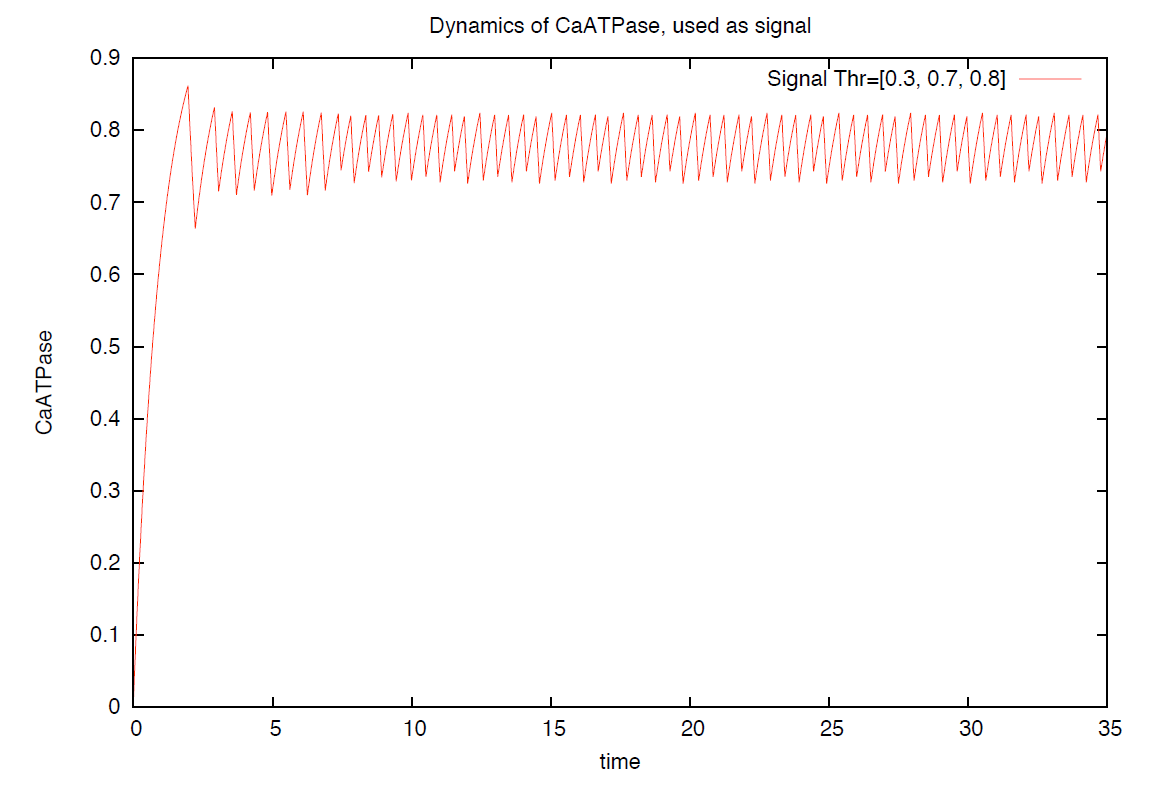
\includegraphics[width=0.9\linewidth]{gfx/original3Nodos}
\caption[Dinámica original $Ca^{2+}ATPase$]{Dinámica original de $Ca^{2+}ATPase$ de las ecucaciones de Glass con parámetros $\alpha_{CIS} = \alpha_{Ca^{2+}} =  \alpha_{Ca^{2+}ATPase} = 1$, umbrales de activación $\theta_{CIS} = 0.3$, $\theta_{Ca^{2+}} = 0.7$ y $\theta_{Ca^{2+}APTase} = 0.8$, y $CIS = 1$, $Ca^{2+} = 0$, $Ca^{2+}ATPase = 0$ como condiciones iniciales.}\label{fig:signal3nodos}
\end{figure}

Se eligió búsqueda aleatoria como estrategia de exploración del espacio de búsqueda, mientras que la función objetivo consistió en minimizar $f_{SI}(X,Y) = 1 -SI(X,Y)$ con $X$ la señal original y $Y$ los datos de la dinámica de Glass del nodo $Ca^{2+}ATPase$ de cada uno de los candidatos propuestos por el algoritmo de búsqueda.

\begin{figure}[hbt]
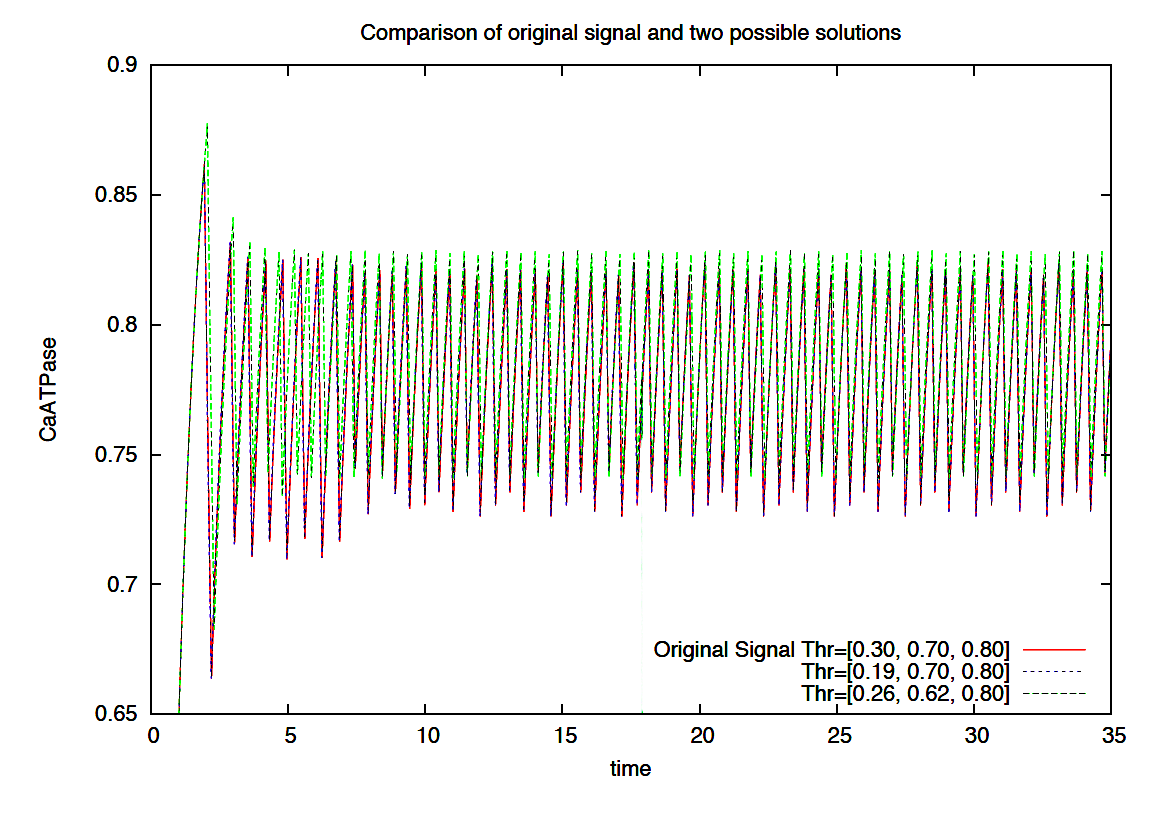
\includegraphics[width=0.9\linewidth]{gfx/comparacion3Nodos}
\caption[Dinámicas original y estimada $Ca^{2+}ATPase$]{Dinámicas original y estimada de $Ca^{2+}ATPase$ de la red de 3 nodos. En rojo la señal original, verde y azul representan dos distintas ejecuciones del programa de búsqueda.}\label{fig:resultadoChido3Nodos}
\end{figure}

En este caso, fue posible recuperar el valor de los tres parámetros en varias ejecuciones del programa de búsqueda. La figura \ref{fig:resultadoChido3Nodos} muestra la dinámica original y el resultado obtenido con dos ejecuciones distintas del programa de busqueda.

Se probó realizar la estimación de parámetros para el mismo sistema usando una versión de algoritmos genéticos adaptada a problemas con variables continuas con los parámetros recomendados por omision, tal como se refiere en \citeauthor{Haupt1998} \citep{Haupt1998}. En este caso fue posible recuperar el valor del parámetro de umbral para $Ca^{2+}ATPase$, si bien con una precisión menor.
% Después tal vez sea bueno agregar los resultados a un apéndice.

Cabe mencionar que a pesar de que este caso de ejemplo no está relacionado en un sentido bioquímico con la red de señalización de speract, sí lo está en términos de ser un modelo discreto que se quiere reescribir como semicontinuo. Además, para la estimación de parámetros se usó un solo tipo de señal o ``medición experimental'' contra la cual comparar la dinámica de cada uno de los candidatos, situación que se presentó también en la red de señalización, donde solo se cuenta con un único tipo de mediciones para tiempos largos. La experiencia ganada con este caso de ejemplo sirvió como base para abordar la estimación de parámetros del modelo semicontinuo de la vía de señalización de speract.

\subsection{Modelo de la red de señalización}

El modelo semicontinuo de la vía de señalización de speract se implementó planteando ecuaciones de Glass cuyo valor depende de un conjunto de funciones discretas, estas últimas basadas en el modelo de \citeauthor{Espinal2011} \citep{Espinal2011}. La implementación en lenguaje C de dichas funciones discretas se muestran en el apéndice \ref{ch:appendix}. A modo de ejemplo, puede considerarse la ecuación de Glass para cGMP. La tabla de verdad de la función discreta se muestra en la tabla \ref{tab:tabla_cGMP}, y la ecuación de Glass correspondiente en la ecuación \ref{eqn:glasscGMP}.

\begin{table}[hb]
    \myfloatalign
  \begin{tabularx}{\textwidth}{cccc} \toprule
    \tableheadline{GC(t)} & \tableheadline{PDE(t)} & \tableheadline{cGMP(t)} & \tableheadline{cGMP(t+1)} \\
	\midrule
	0 &	0 & 0 &	0 \\
	0 & 0 & 1 & 1 \\
	0 & 1 & 0 & 0 \\
	0 & 1 & 1 & 0 \\
	1 & 0 & 0 & 1 \\
	1 & 0 & 1 & 1 \\
	1 & 1 & 0 & 0 \\
	1 & 1 & 1 & 0 \\
    \bottomrule
  \end{tabularx}
  \caption[Tabla de regulación de cGMP]{Tabla de regulación de cGMP}
  \label{tab:tabla_cGMP}
\end{table}

Y la ecuación de Glass correspondiente es:

\begin{equation}\label{eqn:glasscGMP}
\frac{dcGMP}{dt} = \alpha_{cGMP} [F_{cGMP}(\widehat{GC}, \widehat{PDE}, \widehat{cGMP}) - cGMP]
\end{equation}
\\
donde
$$\widehat{GC} = H(GC - \theta_{GC})$$ $$\widehat{PDE} = H(PDE - \theta_{PDE})$$ y $$\widehat{cGMP} = H(cGMP - \theta_{cGMP})$$
\\
son los valores discretizados de las variables continuas $GC$, $PDE$ y $cGMP$, respectivamente.

El problema de estimación de parámetros en este caso consiste en ajustar el valor de 26 parámetros de umbral $\theta_i$ (22 para los nodos binarios y 4 extras para los nodos que tienen un valor terciario), en el caso de un sistema sincronizado donde todos los parámetros $\alpha_i=x$, $x \in [0,T_{max}]$, donde $T_{max}$ es el tiempo característico más grande del sistema. 

Un problema similar, si bien más complicado, es permitir que cada $\alpha_i$ tome un valor distinto de los demás $\alpha_i$, es decir, un problema asíncrono. El problema asíncrono añade la necesidad de estimar 22 parámetros extra, uno para cada componente del sistema.

Como una primera aproximación al problema, se consideró el problema sincronizado, estableciendo $\alpha_i = 1.0\ \forall i$, de modo que solo se debió estimar el valor de los 26 parámetros de umbral. Las condiciones iniciales se fijaron tales que el valor inicial para el potencial de membrana $V = 1.0$, los canales $HVA=LVA=1.0$, $dCA = 0.9$ y el resto con valor $0.2$. Al discretizar estos valores, se tiene una condición inicial muy similar a la del organismo silvestre según el modelo discreto antecedente de este trabajo. 

En vista de que aun para el problema sincronizado el espacio de parámetros es mayor que el del problema de 3 nodos presentado en la sección anterior, y de que los algoritmos genéticos no presentaron una mejora con respecto a la búsqueda aleatoria en el mismo problema, se buscó otro método de exploración del espacio de búsqueda. A este respecto, \citeauthor{BangaMoles2003} \citep{BangaMoles2003} muestran que para problemas de estimación de parámetros en redes de señalización bioquímica los métodos con mejores resultados son aquellos basados en estrategias evolutivas. En especial algunos como Evolución Diferencial resultan aún mejores que los algoritmos genéticos.

Para la búsqueda de parámetros de la vía de señalización de speract se usó entonces Evolución Diferencial como estrategia de búsqueda (y evaluación de candidatos), usando los parámetros recomendados en la literatura \citeauthor{Storn1997}  \citep{Storn1997}. Para comparar la dinámica del nodo de $Ca^{2+}$, (denotado en el modelo como $dCa$) de cada modelo planteado con las mediciones experimentales de fluorescencia de $Ca^{2+}$, se buscó minimizar $f_{Pearson}(X,Y) = 1-r_{X,Y}$, donde $X$ son los datos experimentales y $Y$ son los datos de la dinámica del nodo de calcio del modelo. 

Los sistemas de ecuaciones de Glass se resolvieron mediante el método de Euler. Para algunas dinámicas elegidas por el algoritmo de Evolución Diferencial, se verificó la solución usando el método de Adams-Bashforth. No se encontraron diferencias significativas entre las soluciones de uno y otro métodos.

Se logró ajustar la dinámica del nodo de $Ca^{2+}$ de acuerdo a mediciones experimentales, como se muestra en la figura \ref{fig:glassChido}. 

\begin{figure}[h]
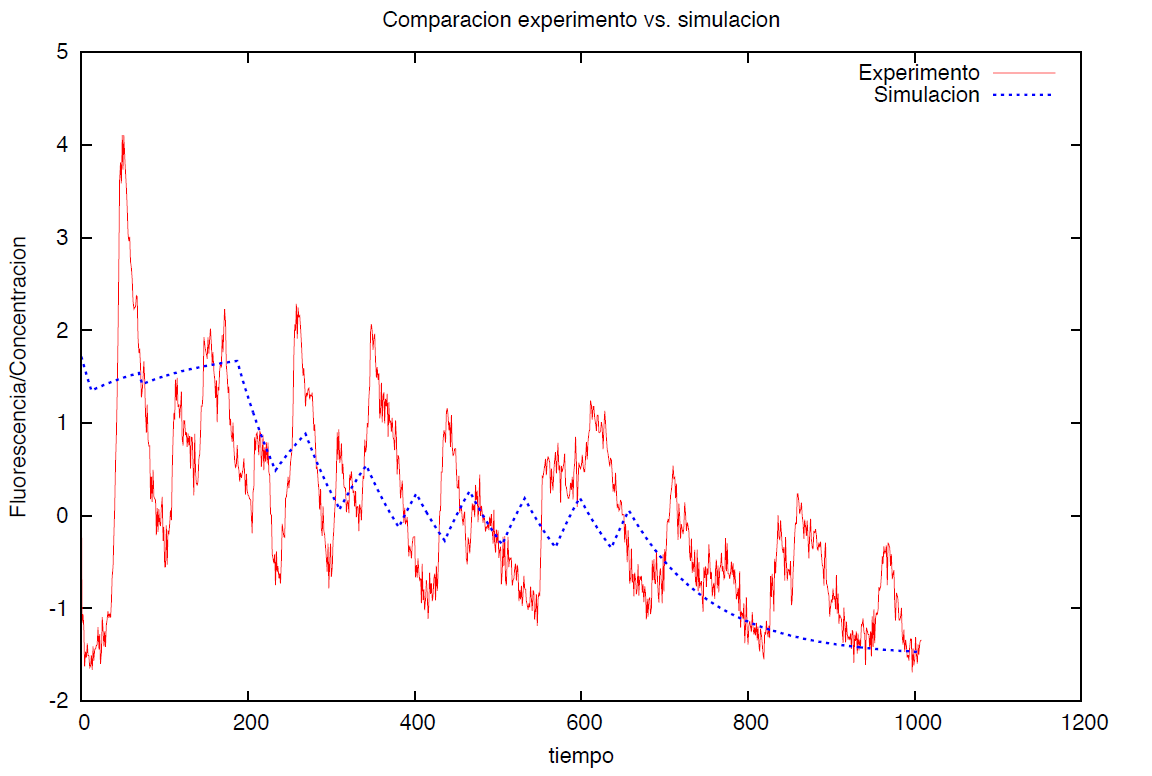
\includegraphics[width=0.9\linewidth]{gfx/glassChido}
\caption[Dinámica del nodo de $Ca^{2+}$ del modelo y medición experimental de $Ca^{2+}$]{Dinámica del nodo de $Ca^{2+}$ del modelo y medición experimental de $Ca^{2+}$. En rojo la medición experimental, en azul el ajuste usando la función objetivo basada en la correlación de Pearson. Para efectos de comparación, las series se normalizaron de manera que tuvieran promedio $0$ y varianza $1$.}\label{fig:glassChido}
\end{figure}

A pesar de lo alentador de este resultado, el comportamiento dinámico de otros nodos aún necesita mayor revisión. Por ejemplo, el nodo correspondiente al potencial de membrana $V$ debería de disminuir su valor al inicio de la dinámica para luego aumentarlo. Sin embargo, el potencial aumenta al principio y disminuye posteriormente. Este comportamiento es imposible en la realidad, ya que al haber un aumento de $[Ca^{2+}]_i$ el potencial deberia disminuir. Véase la figura \ref{fig:glassChafa}.

\begin{figure}[h]
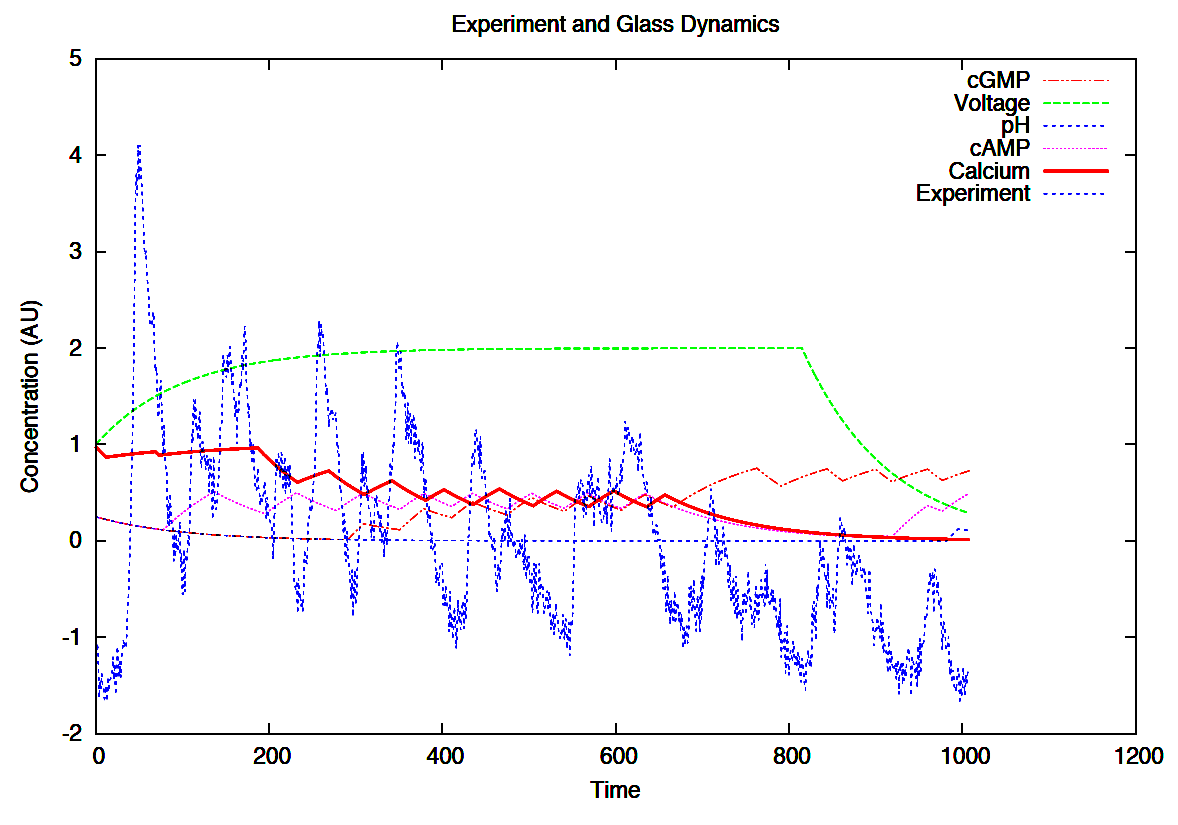
\includegraphics[width=0.9\linewidth]{gfx/glassChafa}
\caption[Dinámica de $Ca^{2+}$, $V$ y otros componentes del modelo, y medición experimental de $Ca^{2+}$]{Dinámica del nodo de $Ca^{2+}$, $V$ y otros componentes del modelo, y medición experimental de $Ca^{2+}$. En este caso en azul punteado se muestra la medición expetimental, en rojo el nodo de $Ca^{2+}$ del modelo y en verde el nodo que representa al potencial de membrana en el modelo. Nótese que se trata de una ejecución del algoritmo de búsqueda distinta a la de la figura \ref{fig:glassChido}. Para efectos de comparación, las series se normalizaron de manera que tuvieran promedio $0$ y varianza $1$.}\label{fig:glassChafa}
\end{figure}

Varias ejecuciones del algoritmo de evolución diferencial, diferentes parámetros para el mismo algoritmo y funciones objetivo distintas, es decir, usando error cuadrático medio \textsc{mse} o el índice de pendiente \textsc{(si)} arrojaron resultados similares.













































%************************************************
\chapter{Conclusiones y Perspectivas}\label{ch:conclusiones}
%************************************************

% While it has not been possible to provide definite answers to the questions (Unsuccessful experiment, but I still hope to get it published)
% Three of the samples were chosen for detailed study (The other results didn't make any sense)
% A highly significant area for exploratory study (A totally useless topic selected by my commitee)
% In my experience / in case after case / in a series of cases
% Correct within an order of magnitude / Can be regarded good within some range of validity
% It is clear that much additional work will be required before a complete understanding of this phenomenon occurs
% It is hoped that this study will stimulate further investigations in this field

Este capítulo presenta algunas conclusiones, y al final menciona ideas que podrían ser de utilidad para extender y refinar la investigación iniciada en este trabajo. 

\section{Conclusiones}

%\paragraph {La transformación de modelos discretos en semicontinuos (ecuaciones de Glass) basada en estimación de parámetros es posible}Se mostró que es posible la transformación de modelos discretos en semicontinuos mediante un ejemplo consistente en una pequeña red Booleana sincronizada compuesta por tres nodos. En este caso solo fue necesario estimar tres parámetros y se contó con un solo tipo de medición ``experimental'' o señal original contra la cual comparar. Para este tipo de problema, la elección de estrategia de búsqueda no tiene mayor consecuencia, ya que es posible obtener resultados satisfactorios aún con la búsqueda aleatoria. El índice de pendiente \textsc{(si)} mostró ser una buena medida de comparación entre señales.  

\paragraph {La transformación de un modelo discreto en semicontinuo produce buenos resultados en sistemas donde la relación \emph{parámetros a estimar}/\emph{tipos de mediciones} es alta}El modelo Booleano de 3 nodos muestra que el paso de un formalismo de modelación a otro puede ser exitoso cuando se cuenta con datos suficientes contra los cuales comparar el modelo, en relación a la cantidad de parámetros a estimar. Por el contrario, en modelos como el de la vía señalización, en los que la cantidad de parámetros es mucho mayor que los criterios contra los cuales comparar, es difícil encontrar resultados biológicamente relevantes.

\paragraph {La elección de parámetros para modelos de Glass no es simple} A pesar del éxito que han tenido algunos modelos (\citeauthor{AlvarezBuylla:2008cg} \citep{AlvarezBuylla:2008cg}, \citeauthor{Azpeitia:2010ik} \citep{Azpeitia:2010ik}) en reproducir el comportamiento observado experimentalmente, este trabajo muestra que no siempre es directo encontrar un conjunto de parámetros tales que la dinámica del modelo tenga una interpretación biológica correcta. Establecer los inversos de tiempo característicos en un valor de $1$ y los umbrales de cada nodo en $0.5$ parece ser una buena primera elección ante falta de información detallada, pero no necesariamente es correcta en todos los casos.

\paragraph {Es necesaria una metodología general para la transformación de modelos discretos en modelos de ecuaciones de Glass} La metodología empleada en este trabajo no presenta una forma generalizada para la transformación de modelos discretos en semicontinuos basados en ecuaciones de Glass. Este tipo de modelos resultan atractivos puesto que constituyen un paso intermedio entre los modelos discretos, que requieren poca información, y los basados en ecuaciones diferenciales, que requieren más información detallada. Contar con una metodología generalizada permitiría construir de manera semiautomática una representación más detallada del sistema que la de un modelo discreto, a partir de apenas un poco más de información que la usada para construir a este último pero sin llegar al nivel de detalle requerido por un modelo de ecuaciones diferenciales ordinarias.

\section{Perspectivas y trabajo futuro}

Este trabajo se desarrolló bajo el supuesto de que la transformación de modelos discretos en semicontinuos podía realizarse mediante el empleo de técnicas de estimación de parámetros, particularmente aquellas basadas en estrategias evolutivas. Las funciones objetivo utilizadas se basan en criterios simples de correlación o minimización de diferencias. 

Existe un marco teórico más desarrollado para la solución de problemas inversos, que cuenta con técnicas elaboradas para el problema de discriminación de modelos. Una técnica que puede resultar prometedora para la solución de este tipo de problemas puede ser la \textsc{Regularización Promotora de Dispersión o Sparsity Enforcing Regularization}, \citeauthor{Engl2009} \citep{Engl2009}, en donde se busca hacer uso de criterios estadísticos para la comparación entre mediciones experimentales y modelos.

Otra posibilidad que valdría la pena explorar consiste en modificar el modelo discreto de modo que contenga menos nodos y por lo tanto haya menos parámetros que estimar. Hasta este momento cuál es un buen criterio general de reducción de modelos discretos sigue siendo una pregunta abierta. Sin embargo, se ha explorado la posibilidad de utilizar criterios de robustez de las redes para separar nodos esenciales para mantener la dinámica y función de la red de aquellos nodos que podrían parecer redundantes.

Usando este último criterio, se ha logrado plantear un modelo discreto de la vía de señalización de speract con 11 nodos. Queda abierto el determinar si a partir de este modelo reducido y los datos experimentales con que se cuenta hasta el momento, es posible ajustar el comportamiento de un modelo semicontinuo de manera que la interpretación biológica del modelo sea más completa que lo alcanzado hasta el momento.

%Una alternativa a otro tipo de comparaciones es la \textsc{Regularización Promotora de Dispersión o Sparsity Promoting Regularization}, \citeauthor{Engl2009}. La idea consiste en imputar un modelo estadístico a la comparación de mediciones experimentales con modelos de ecuaciones diferenciales. Los operadores diferenciales que no incluyen componentes estocásticos suelen producir trayectorias por lo general suaves, en contraste con la variabilidad existente en las series de tiempo de las mediciones experimentales. 
%
%Sea $\mathbf{p}$ el vector de parámetros de un conjunto de ecuaciones diferenciales. Sea $\Phi(\mathbf{p},t)$ la trayectoria solución dependiente del tiempo $t$ y del vector de parámetros $\mathbf{p}$. Sea $\Psi(\Phi(\mathbf{p},t))$ un modelo Gaussiano del ruido de las mediciones experimentales con desviación estándar constante. El objetivo de añadir $\Phi$  es imputar un criterio estadístico a la trayectoria solución de la ecuación diferencial, y hacer entonces una comparación entre un modelo estadísticos y un conjunto de datos.

% It is hoped that this study will stimulate further investigations in this field


%\include{multiToC} % <--- just debug stuff, ignore for your documents
% ********************************************************************
% Backmatter
%*******************************************************
\appendix
\cleardoublepage
%\part{Appendix}
%********************************************************************
% Appendix
%*******************************************************
% If problems with the headers: get headings in appendix etc. right
%\markboth{\spacedlowsmallcaps{Appendix}}{\spacedlowsmallcaps{Appendix}}
\chapter{Apéndice}\label{ch:appendix}

\begin{lstlisting}[caption=Modelo discreto de la vía de señalización. Implementación en C]

#include "discreteFunction.h"

int
voltage [72][2] ={
	{0,	1},
	{1,	1},
	{2,	2},
	{3,	2},
	{4,	2},
	{5,	2},
	{9,	2},
	{10,	2},
	{11,	2},
	{12,	2},
	{13,	2},
	{14,	2},
	{18,	2},
	{19,	2},
	{20,	2},
	{21,	2},
	{22,	2},
	{23,	2},
	{27,	0},
	{28,	0},
	{29,	0},
	{30,	1},
	{31,	2},
	{32,	1},
	{36,	2},
	{37,	2},
	{38,	1},
	{39,	2},
	{40,	2},
	{41,	1},
	{45,	2},
	{46,	1},
	{47,	1},
	{48,	2},
	{49,	2},
	{50,	1},
	{81,	0},
	{82,	0},
	{83,	0},
	{84,	2},
	{85,	1},
	{86,	1},
	{90,	2},
	{91,	2},
	{92,	0},
	{93,	2},
	{94,	2},
	{95,	1},
	{99,	2},
	{100,	2},
	{101,	0},
	{102,	2},
	{103,	2},
	{104,	1},
	{108,	0},
	{109,	0},
	{110,	0},
	{111,	0},
	{112,	0},
	{113,	0},
	{117,	2},
	{118,	0},
	{119,	0},
	{120,	1},
	{121,	1},
	{122,	1},
	{126,	1},
	{127,	0},
	{128,	0},
	{129,	1},
	{130,	1},
	{131,	1}
};

int 
calcium [432][2] =
{	
	{0,	0},
	{1,	0},
	{2,	0},
	{3,	0},
	{4,	0},
	{5,	0},
	{9,	0},
	{10,	0},
	{11,	0},
	{12,	0},
	{13,	0},	
	{14,	0},
	{27,	0},
	{28,	0},
	{29,	0},
	{30,	0},
	{31,	0},
	{32,	0},
	{36,	0},
	{37,	0},	
	{38,	0},
	{39,	0},
	{40,	0},
	{41,	0},
	{81,	0},
	{82,	0},
	{83,	0},
	{84,	0},
	{85,	0},	
	{86,	0},
	{90,	0},
	{91,	0},
	{92,	0},
	{93,	0},
	{94,	0},
	{95,	0},
	{108,	0},
	{109,	0},
	{110,	0},
	{111,	0},
	{112,	0},
	{113,	0},
	{117,	0},
	{118,	0},
	{119,	0},
	{120,	0},
	{121,	0},
	{122,	0},
	{162,	0},
	{163,	0},
	{164,	0},
	{165,	0},
	{166,	0},
	{167,	0},
	{171,	0},
	{172,	0},
	{173,	0},
	{174,	0},
	{175,	0},
	{176,	0},
	{189,	0},
	{190,	0},
	{191,	0},
	{192,	0},
	{193,	0},
	{194,	0},
	{198,	0},
	{199,	0},
	{200,	0},
	{201,	0},
	{202,	0},
	{203,	0},
	{243,	0},
	{244,	0},
	{245,	1},
	{246,	0},
	{247,	0},
	{248,	1},
	{252,	0},
	{253,	0},
	{254,	1},
	{255,	0},
	{256,	0},
	{257,	0},
	{270,	1},
	{271,	1},
	{272,	1},
	{273,	1},
	{274,	1},
	{275,	1},
	{279,	1},
	{280,	1},
	{281,	1},
	{282,	0},
	{283,	0},
	{284,	1},
	{324,	0},
	{325,	0},
	{326,	1},
	{327,	0},
	{328,	0},
	{329,	1},
	{333,	0},
	{334,	0},
	{335,	1},
	{336,	0},
	{337,	0},
	{338,	0},
	{351,	1},
	{352,	1},
	{353,	1},
	{354,	1},
	{355,	1},
	{356,	1},
	{360,	1},
	{361,	1},
	{362,	1},
	{363,	0},
	{364,	0},
	{365,	1},
	{405,	2},
	{406,	2},
	{407,	2},
	{408,	2},
	{409,	2},
	{410,	2},
	{414,	2},
	{415,	2},
	{416,	2},
	{417,	2},
	{418,	2},
	{419,	2},
	{432,	2},
	{433,	2},
	{434,	2},
	{435,	2},
	{436,	2},
	{437,	2},
	{441,	2},
	{442,	2},
	{443,	2},
	{444,	2},
	{445,	2},
	{446,	2},
	{729,	0},
	{730,	0},
	{731,	0},
	{732,	0},
	{733,	0},
	{734,	0},
	{738,	0},
	{739,	0},
	{740,	0},
	{741,	0},
	{742,	0},
	{743,	0},
	{756,	0},
	{757,	0},
	{758,	0},
	{759,	0},
	{760,	0},
	{761,	0},
	{765,	0},
	{766,	0},
	{767,	0},
	{768,	0},
	{769,	0},
	{770,	0},
	{810,	0},
	{811,	0},
	{812,	0},
	{813,	0},
	{814,	0},
	{815,	0},
	{819,	0},
	{820,	0},
	{821,	0},
	{822,	0},
	{823,	0},
	{824,	0},
	{837,	0},
	{838,	0},
	{839,	0},
	{840,	0},
	{841,	0},
	{842,	0},
	{846,	0},
	{847,	0},
	{848,	0},
	{849,	0},
	{850,	0},
	{851,	0},
	{891,	0},
	{892,	0},
	{893,	0},
	{894,	0},
	{895,	0},
	{896,	0},
	{900,	0},
	{901,	0},
	{902,	0},
	{903,	0},
	{904,	0},
	{905,	0},
	{918,	0},
	{919,	0},
	{920,	0},
	{921,	0},
	{922,	0},
	{923,	0},
	{927,	0},
	{928,	0},
	{929,	0},
	{930,	0},
	{931,	0},
	{932,	0},
	{972,	1},
	{973,	1},
	{974,	1},
	{975,	0},
	{976,	0},
	{977,	1},
	{981,	0},
	{982,	0},
	{983,	1},
	{984,	0},
	{985,	0},
	{986,	0},
	{999,	1},
	{1000,	1},
	{1001,	1},
	{1002,	1},
	{1003,	1},
	{1004,	1},
	{1008,	1},
	{1009,	1},
	{1010,	1},
	{1011,	0},
	{1012,	0},
	{1013,	1},
	{1053,	1},
	{1054,	1},
	{1055,	1},
	{1056,	0},
	{1057,	0},
	{1058,	1},
	{1062,	0},
	{1063,	0},
	{1064,	1},
	{1065,	0},
	{1066,	0},
	{1067,	0},
	{1080,	1},
	{1081,	1},
	{1082,	1},
	{1083,	1},
	{1084,	1},
	{1085,	1},
	{1089,	1},
	{1090,	1},
	{1091,	1},
	{1092,	0},
	{1093,	0},
	{1094,	1},
	{1134,	2},
	{1135,	2},
	{1136,	2},
	{1137,	2},
	{1138,	2},
	{1139,	2},
	{1143,	2},
	{1144,	2},
	{1145,	2},
	{1146,	2},
	{1147,	2},
	{1148,	2},
	{1161,	2},
	{1162,	2},
	{1163,	2},
	{1164,	2},
	{1165,	2},
	{1166,	2},
	{1170,	2},
	{1171,	2},
	{1172,	2},
	{1173,	2},
	{1174,	2},
	{1175,	2},
	{1458,	0},
	{1459,	0},
	{1460,	0},
	{1461,	0},
	{1462,	0},
	{1463,	0},
	{1467,	0},
	{1468,	0},
	{1469,	0},
	{1470,	0},
	{1471,	0},
	{1472,	0},
	{1485,	0},
	{1486,	0},
	{1487,	0},
	{1488,	0},
	{1489,	0},
	{1490,	0},
	{1494,	0},
	{1495,	0},
	{1496,	0},
	{1497,	0},
	{1498,	0},
	{1499,	0},
	{1539,	0},
	{1540,	0},
	{1541,	0},
	{1542,	0},
	{1543,	0},
	{1544,	0},
	{1548,	0},
	{1549,	0},
	{1550,	0},
	{1551,	0},
	{1552,	0},
	{1553,	0},
	{1566,	0},
	{1567,	0},
	{1568,	0},
	{1569,	0},
	{1570,	0},
	{1571,	0},
	{1575,	0},
	{1576,	0},
	{1577,	0},
	{1578,	0},
	{1579,	0},
	{1580,	0},
	{1620,	0},
	{1621,	0},
	{1622,	0},
	{1623,	0},
	{1624,	0},
	{1625,	0},
	{1629,	0},
	{1630,	0},
	{1631,	0},
	{1632,	0},
	{1633,	0},
	{1634,	0},
	{1647,	0},
	{1648,	0},
	{1649,	0},
	{1650,	0},
	{1651,	0},
	{1652,	0},
	{1656,	0},
	{1657,	0},
	{1658,	0},
	{1659,	0},
	{1660,	0},
	{1661,	0},
	{1701,	1},
	{1702,	1},
	{1703,	1},
	{1704,	1},
	{1705,	1},
	{1706,	1},
	{1710,	1},
	{1711,	1},
	{1712,	1},
	{1713,	1},
	{1714,	1},
	{1715,	1},
	{1728,	2},
	{1729,	2},
	{1730,	1},
	{1731,	1},
	{1732,	1},
	{1733,	1},
	{1737,	1},
	{1738,	1},
	{1739,	1},
	{1740,	1},
	{1741,	1},
	{1742,	1},
	{1782,	1},
	{1783,	1},
	{1784,	1},
	{1785,	1},
	{1786,	1},
	{1787,	1},
	{1791,	1},
	{1792,	1},
	{1793,	1},
	{1794,	1},
	{1795,	1},
	{1796,	1},
	{1809,	1},
	{1810,	1},
	{1811,	1},
	{1812,	1},
	{1813,	1},
	{1814,	1},
	{1818,	1},
	{1819,	1},
	{1820,	1},
	{1821,	1},
	{1822,	1},
	{1823,	1},
	{1863,	2},
	{1864,	2},
	{1865,	2},
	{1866,	2},
	{1867,	2},
	{1868,	2},
	{1872,	1},
	{1873,	1},
	{1874,	1},
	{1875,	1},
	{1876,	1},
	{1877,	1},
	{1890,	1},
	{1891,	1},
	{1892,	1},
	{1893,	1},
	{1894,	1},
	{1895,	1},
	{1899,	1},
	{1900,	1},
	{1901,	1},
	{1902,	1},
	{1903,	1},
	{1904,	1}
};

int compareints (const void * a, const void * b)
{
	return ( *(int*)a - *(int*)b );
}
 
int discreteModel (const int i, const int * st)
{
	// Nodo 26_CaKC es st[19]
	// Nodo 22_PDE es st[21]
	int rvalue = 0;
	int *pItem;
	int key;
	switch (i) {
		case 0: //sr
			rvalue = 1;
			break;
		case 1: //GC
			rvalue = ( (st[0]==1) && (st[11]==0) ) ? 1 : 0;
			break;
		case 2: //cGMP
			rvalue = ( (st[1]==0 && st[21]==0 && st[2]==1) || (st[1]==1 && st[21]==0 && st[2]==0) || (st[1]==1 && st[21]==0 && st[2]==1) ) ? 1 : 0;
			break;
		case 3: //KCNG
			rvalue = (st[2]==1) ? 1 : 0;
			break;
		case 4: //pK
			rvalue = (st[3]==0 && st[19]==0) ? 0 : 1;
			break;
		case 5: //v
			// Transform the key form ternary to decimal representation. Use that key to lookup in the table
			key = (st[4]*81) + (st[20]*27) + (st[15]*9) + (st[12]*3) + st[5];			
			pItem = (int*) bsearch (&key, voltage, 72, sizeof (int *), compareints);
			if (pItem!=NULL)
				rvalue = *(pItem+1);
			else {
				fprintf(stderr, "Bad regulator configuration at node index %d at function %s, file %s, line %d\nAborting...\n", i, __func__, __FILE__, __LINE__);
				fprintf(stderr, "Offending configuration is = %d, %d, %d, %d, %d\n", st[4], st[20], st[15], st[12], st[5] );
			}
			break;
		case 6: //NHE
			rvalue = (st[5]==0 && st[11]==0) ? 1 : 0;
			break;
		case 7: //NCE
			rvalue = ( (st[5]==0 && st[15]==0) || (st[5]==0 && st[15]==1) || (st[5]==0 && st[15]==2) ) ? 1 : 0;
			break;
		case 8: //HCN
			rvalue = ( (st[5]==0 && st[13]==0) || (st[5]==0 && st[13]==1) ) ? 1 : 0;
			break;
		case 9: //AC
			rvalue = ((st[5]==1 && st[11]==0 && st[15]==0) || (st[5]==1 && st[11]==0 && st[15]==1) ||
					  (st[5]==1 && st[11]==1 && st[15]==0) || (st[5]==2 && st[11]==0 && st[15]==0) ||
					  (st[5]==2 && st[11]==0 && st[15]==1) || (st[5]==2 && st[11]==1 && st[15]==0) ||
					  (st[5]==2 && st[11]==1 && st[15]==1) ) ? 0 : 1;
			break;
		case 10: //LVA
			if ((st[5]==0 && st[10]==0) || (st[5]==0 && st[10]==1) || (st[5]==1 && st[10]==1) ){
				rvalue = 1;
			}else if (st[5]==2 && st[10]==1) {
				rvalue = 2;
			}else {
				rvalue = 0;
			}
			break;
		case 11: //uPH
			rvalue = (st[6]==0) ? 0 : 1;
			break;
		case 12: //pNa
			rvalue = (st[8]==0) ? 0 : 1;
			break;
		case 13: //cAMP
			rvalue = ( (st[9]==0 && st[21]==0 && st[13]==1) || (st[9]==1 && st[21]==0 && st[13]==0) || (st[9]==1 && st[21]==0 && st[13]==1) ) ? 1 : 0;
			break;
		case 14: //HVA
			if ( (st[5]==0 && st[14]==0) || (st[5]==0 && st[14]==1) ) {
				rvalue = 1;
			}else if ((st[5]==0 && st[14]==2) || (st[5]==1 && st[14]==0) || (st[5]==2 && st[14]==0)) {
				rvalue = 0;
			}else {
				rvalue = 2;
			}
			break;
		case 15: //pCa
			key = (st[15]*729) + (st[0]*243) + (st[10]*81) + (st[18]*27) + (st[7]*9) + (st[16]*3) + st[14];
			pItem = (int*) bsearch (&key, calcium, 432, sizeof (int *), compareints);
			if (pItem!=NULL)
				rvalue = *(pItem+1);
			else
				fprintf(stderr, "Bad regulator configuration at node index %d at function %s, file %s, line %d\nAborting...\n", i, __func__, __FILE__, __LINE__);
			break;
		case 16: //CaP
			rvalue = (st[15]==0) ? 0 : 1;
			break;
		case 17: //CaCC
			rvalue = (st[15]==0) ? 0 : 1;
			break;
		case 18: //cAMPCC
			rvalue = (st[13]==0) ? 0 : 1;
			break;
		case 19: //CaKC
			rvalue = ( (st[15]==1 && st[5]==2) || (st[15]==2 && st[5]==2) ) ? 1 : 0;
			break;
		case 20: //pCl
			rvalue = (st[17]==0) ? 0 : 1;
			break;
		case 21: //PDE
			rvalue = (st[2]==0 && st[13]==0) ? 0 : 1;
			break;
		default:
			fprintf(stderr, "Bad node index %d at function %s, file %s, line %d\nAborting...\n", i, __func__, __FILE__, __LINE__);
			break;
	}
	return rvalue;

\end{lstlisting}

%\begin{table}
%    \myfloatalign
%  \begin{tabularx}{\textwidth}{Xll} \toprule
%    \tableheadline{labitur bonorum pri no} & \tableheadline{que vista}
%    & \tableheadline{human} \\ \midrule
%    fastidii ea ius & germano &  demonstratea \\
%    suscipit instructior & titulo & personas \\
%    %postulant quo & westeuropee & sanctificatec \\
%    \midrule
%    quaestio philosophia & facto & demonstrated \\
%    %autem vulputate ex & parola & romanic \\
%    %usu mucius iisque & studio & sanctificatef \\
%    \bottomrule
%  \end{tabularx}
%  \caption[Autem usu id]{Autem usu id.}
%  \label{tab:moreexample}
%\end{table}
%
%Ei solet nemore consectetuer nam. Ad eam porro impetus, te choro omnes
%evertitur mel. Molestie conclusionemque vel at, no qui omittam
%expetenda efficiendi. Eu quo nobis offendit, verterem scriptorem ne
%vix.
%
%  
%\begin{lstlisting}[float,caption=A floating example]
%for i:=maxint to 0 do
%begin
%{ do nothing }
%end;
%\end{lstlisting}
%%********************************************************************
% Appendix
%*******************************************************
% If problems with the headers: get headings in appendix etc. right
%\markboth{\spacedlowsmallcaps{Appendix}}{\spacedlowsmallcaps{Appendix}}
\chapter{Código}\label{ch:appendix}

\begin{lstlisting}[caption=Modelo discreto de la vía de señalización. Implementación en C]

#include "discreteFunction.h"

int
voltage [72][2] ={
	{0,1},{1,1},{2,2},{3,2},{4,2},{5,2},{9,2},{10,2},
	{11,2},{12,2},{13,2},{14,2},{18,2},{19,2},{20,2},{21,2},{22,2},{23,2},
	{27,0},
	{28,0},
	{29,0},
	{30,1},
	{31,2},
	{32,1},
	{36,2},
	{37,2},
	{38,1},
	{39,2},
	{40,2},
	{41,1},
	{45,2},
	{46,	1},
	{47,	1},
	{48,	2},
	{49,	2},
	{50,	1},
	{81,	0},
	{82,	0},
	{83,	0},
	{84,	2},
	{85,	1},
	{86,	1},
	{90,	2},
	{91,	2},
	{92,	0},
	{93,	2},
	{94,	2},
	{95,	1},
	{99,	2},
	{100,	2},
	{101,	0},
	{102,	2},
	{103,	2},
	{104,	1},
	{108,	0},
	{109,	0},
	{110,	0},
	{111,	0},
	{112,	0},
	{113,	0},
	{117,	2},
	{118,	0},
	{119,	0},
	{120,	1},
	{121,	1},
	{122,	1},
	{126,	1},
	{127,	0},
	{128,	0},
	{129,	1},
	{130,	1},
	{131,	1}
};

int 
calcium [432][2] =
{	
	{0,	0},
	{1,	0},
	{2,	0},
	{3,	0},
	{4,	0},
	{5,	0},
	{9,	0},
	{10,	0},
	{11,	0},
	{12,	0},
	{13,	0},	
	{14,	0},
	{27,	0},
	{28,	0},
	{29,	0},
	{30,	0},
	{31,	0},
	{32,	0},
	{36,	0},
	{37,	0},	
	{38,	0},
	{39,	0},
	{40,	0},
	{41,	0},
	{81,	0},
	{82,	0},
	{83,	0},
	{84,	0},
	{85,	0},	
	{86,	0},
	{90,	0},
	{91,	0},
	{92,	0},
	{93,	0},
	{94,	0},
	{95,	0},
	{108,	0},
	{109,	0},
	{110,	0},
	{111,	0},
	{112,	0},
	{113,	0},
	{117,	0},
	{118,	0},
	{119,	0},
	{120,	0},
	{121,	0},
	{122,	0},
	{162,	0},
	{163,	0},
	{164,	0},
	{165,	0},
	{166,	0},
	{167,	0},
	{171,	0},
	{172,	0},
	{173,	0},
	{174,	0},
	{175,	0},
	{176,	0},
	{189,	0},
	{190,	0},
	{191,	0},
	{192,	0},
	{193,	0},
	{194,	0},
	{198,	0},
	{199,	0},
	{200,	0},
	{201,	0},
	{202,	0},
	{203,	0},
	{243,	0},
	{244,	0},
	{245,	1},
	{246,	0},
	{247,	0},
	{248,	1},
	{252,	0},
	{253,	0},
	{254,	1},
	{255,	0},
	{256,	0},
	{257,	0},
	{270,	1},
	{271,	1},
	{272,	1},
	{273,	1},
	{274,	1},
	{275,	1},
	{279,	1},
	{280,	1},
	{281,	1},
	{282,	0},
	{283,	0},
	{284,	1},
	{324,	0},
	{325,	0},
	{326,	1},
	{327,	0},
	{328,	0},
	{329,	1},
	{333,	0},
	{334,	0},
	{335,	1},
	{336,	0},
	{337,	0},
	{338,	0},
	{351,	1},
	{352,	1},
	{353,	1},
	{354,	1},
	{355,	1},
	{356,	1},
	{360,	1},
	{361,	1},
	{362,	1},
	{363,	0},
	{364,	0},
	{365,	1},
	{405,	2},
	{406,	2},
	{407,	2},
	{408,	2},
	{409,	2},
	{410,	2},
	{414,	2},
	{415,	2},
	{416,	2},
	{417,	2},
	{418,	2},
	{419,	2},
	{432,	2},
	{433,	2},
	{434,	2},
	{435,	2},
	{436,	2},
	{437,	2},
	{441,	2},
	{442,	2},
	{443,	2},
	{444,	2},
	{445,	2},
	{446,	2},
	{729,	0},
	{730,	0},
	{731,	0},
	{732,	0},
	{733,	0},
	{734,	0},
	{738,	0},
	{739,	0},
	{740,	0},
	{741,	0},
	{742,	0},
	{743,	0},
	{756,	0},
	{757,	0},
	{758,	0},
	{759,	0},
	{760,	0},
	{761,	0},
	{765,	0},
	{766,	0},
	{767,	0},
	{768,	0},
	{769,	0},
	{770,	0},
	{810,	0},
	{811,	0},
	{812,	0},
	{813,	0},
	{814,	0},
	{815,	0},
	{819,	0},
	{820,	0},
	{821,	0},
	{822,	0},
	{823,	0},
	{824,	0},
	{837,	0},
	{838,	0},
	{839,	0},
	{840,	0},
	{841,	0},
	{842,	0},
	{846,	0},
	{847,	0},
	{848,	0},
	{849,	0},
	{850,	0},
	{851,	0},
	{891,	0},
	{892,	0},
	{893,	0},
	{894,	0},
	{895,	0},
	{896,	0},
	{900,	0},
	{901,	0},
	{902,	0},
	{903,	0},
	{904,	0},
	{905,	0},
	{918,	0},
	{919,	0},
	{920,	0},
	{921,	0},
	{922,	0},
	{923,	0},
	{927,	0},
	{928,	0},
	{929,	0},
	{930,	0},
	{931,	0},
	{932,	0},
	{972,	1},
	{973,	1},
	{974,	1},
	{975,	0},
	{976,	0},
	{977,	1},
	{981,	0},
	{982,	0},
	{983,	1},
	{984,	0},
	{985,	0},
	{986,	0},
	{999,	1},
	{1000,	1},
	{1001,	1},
	{1002,	1},
	{1003,	1},
	{1004,	1},
	{1008,	1},
	{1009,	1},
	{1010,	1},
	{1011,	0},
	{1012,	0},
	{1013,	1},
	{1053,	1},
	{1054,	1},
	{1055,	1},
	{1056,	0},
	{1057,	0},
	{1058,	1},
	{1062,	0},
	{1063,	0},
	{1064,	1},
	{1065,	0},
	{1066,	0},
	{1067,	0},
	{1080,	1},
	{1081,	1},
	{1082,	1},
	{1083,	1},
	{1084,	1},
	{1085,	1},
	{1089,	1},
	{1090,	1},
	{1091,	1},
	{1092,	0},
	{1093,	0},
	{1094,	1},
	{1134,	2},
	{1135,	2},
	{1136,	2},
	{1137,	2},
	{1138,	2},
	{1139,	2},
	{1143,	2},
	{1144,	2},
	{1145,	2},
	{1146,	2},
	{1147,	2},
	{1148,	2},
	{1161,	2},
	{1162,	2},
	{1163,	2},
	{1164,	2},
	{1165,	2},
	{1166,	2},
	{1170,	2},
	{1171,	2},
	{1172,	2},
	{1173,	2},
	{1174,	2},
	{1175,	2},
	{1458,	0},
	{1459,	0},
	{1460,	0},
	{1461,	0},
	{1462,	0},
	{1463,	0},
	{1467,	0},
	{1468,	0},
	{1469,	0},
	{1470,	0},
	{1471,	0},
	{1472,	0},
	{1485,	0},
	{1486,	0},
	{1487,	0},
	{1488,	0},
	{1489,	0},
	{1490,	0},
	{1494,	0},
	{1495,	0},
	{1496,	0},
	{1497,	0},
	{1498,	0},
	{1499,	0},
	{1539,	0},
	{1540,	0},
	{1541,	0},
	{1542,	0},
	{1543,	0},
	{1544,	0},
	{1548,	0},
	{1549,	0},
	{1550,	0},
	{1551,	0},
	{1552,	0},
	{1553,	0},
	{1566,	0},
	{1567,	0},
	{1568,	0},
	{1569,	0},
	{1570,	0},
	{1571,	0},
	{1575,	0},
	{1576,	0},
	{1577,	0},
	{1578,	0},
	{1579,	0},
	{1580,	0},
	{1620,	0},
	{1621,	0},
	{1622,	0},
	{1623,	0},
	{1624,	0},
	{1625,	0},
	{1629,	0},
	{1630,	0},
	{1631,	0},
	{1632,	0},
	{1633,	0},
	{1634,	0},
	{1647,	0},
	{1648,	0},
	{1649,	0},
	{1650,	0},
	{1651,	0},
	{1652,	0},
	{1656,	0},
	{1657,	0},
	{1658,	0},
	{1659,	0},
	{1660,	0},
	{1661,	0},
	{1701,	1},
	{1702,	1},
	{1703,	1},
	{1704,	1},
	{1705,	1},
	{1706,	1},
	{1710,	1},
	{1711,	1},
	{1712,	1},
	{1713,	1},
	{1714,	1},
	{1715,	1},
	{1728,	2},
	{1729,	2},
	{1730,	1},
	{1731,	1},
	{1732,	1},
	{1733,	1},
	{1737,	1},
	{1738,	1},
	{1739,	1},
	{1740,	1},
	{1741,	1},
	{1742,	1},
	{1782,	1},
	{1783,	1},
	{1784,	1},
	{1785,	1},
	{1786,	1},
	{1787,	1},
	{1791,	1},
	{1792,	1},
	{1793,	1},
	{1794,	1},
	{1795,	1},
	{1796,	1},
	{1809,	1},
	{1810,	1},
	{1811,	1},
	{1812,	1},
	{1813,	1},
	{1814,	1},
	{1818,	1},
	{1819,	1},
	{1820,	1},
	{1821,	1},
	{1822,	1},
	{1823,	1},
	{1863,	2},
	{1864,	2},
	{1865,	2},
	{1866,	2},
	{1867,	2},
	{1868,	2},
	{1872,	1},
	{1873,	1},
	{1874,	1},
	{1875,	1},
	{1876,	1},
	{1877,	1},
	{1890,	1},
	{1891,	1},
	{1892,	1},
	{1893,	1},
	{1894,	1},
	{1895,	1},
	{1899,	1},
	{1900,	1},
	{1901,	1},
	{1902,	1},
	{1903,	1},
	{1904,	1}
};

int compareints (const void * a, const void * b)
{
	return ( *(int*)a - *(int*)b );
}
 
int discreteModel (const int i, const int * st)
{
	// Nodo 26_CaKC es st[19]
	// Nodo 22_PDE es st[21]
	int rvalue = 0;
	int *pItem;
	int key;
	switch (i) {
		case 0: //sr
			rvalue = 1;
			break;
		case 1: //GC
			rvalue = ( (st[0]==1) && (st[11]==0) ) ? 1 : 0;
			break;
		case 2: //cGMP
			rvalue = ( (st[1]==0 && st[21]==0 && st[2]==1) || (st[1]==1 && st[21]==0 && st[2]==0) || (st[1]==1 && st[21]==0 && st[2]==1) ) ? 1 : 0;
			break;
		case 3: //KCNG
			rvalue = (st[2]==1) ? 1 : 0;
			break;
		case 4: //pK
			rvalue = (st[3]==0 && st[19]==0) ? 0 : 1;
			break;
		case 5: //v
			// Transform the key form ternary to decimal representation. Use that key to lookup in the table
			key = (st[4]*81) + (st[20]*27) + (st[15]*9) + (st[12]*3) + st[5];			
			pItem = (int*) bsearch (&key, voltage, 72, sizeof (int *), compareints);
			if (pItem!=NULL)
				rvalue = *(pItem+1);
			else {
				fprintf(stderr, "Bad regulator configuration at node index %d at function %s, file %s, line %d\nAborting...\n", i, __func__, __FILE__, __LINE__);
				fprintf(stderr, "Offending configuration is = %d, %d, %d, %d, %d\n", st[4], st[20], st[15], st[12], st[5] );
			}
			break;
		case 6: //NHE
			rvalue = (st[5]==0 && st[11]==0) ? 1 : 0;
			break;
		case 7: //NCE
			rvalue = ( (st[5]==0 && st[15]==0) || (st[5]==0 && st[15]==1) || (st[5]==0 && st[15]==2) ) ? 1 : 0;
			break;
		case 8: //HCN
			rvalue = ( (st[5]==0 && st[13]==0) || (st[5]==0 && st[13]==1) ) ? 1 : 0;
			break;
		case 9: //AC
			rvalue = ((st[5]==1 && st[11]==0 && st[15]==0) || (st[5]==1 && st[11]==0 && st[15]==1) ||
					  (st[5]==1 && st[11]==1 && st[15]==0) || (st[5]==2 && st[11]==0 && st[15]==0) ||
					  (st[5]==2 && st[11]==0 && st[15]==1) || (st[5]==2 && st[11]==1 && st[15]==0) ||
					  (st[5]==2 && st[11]==1 && st[15]==1) ) ? 0 : 1;
			break;
		case 10: //LVA
			if ((st[5]==0 && st[10]==0) || (st[5]==0 && st[10]==1) || (st[5]==1 && st[10]==1) ){
				rvalue = 1;
			}else if (st[5]==2 && st[10]==1) {
				rvalue = 2;
			}else {
				rvalue = 0;
			}
			break;
		case 11: //uPH
			rvalue = (st[6]==0) ? 0 : 1;
			break;
		case 12: //pNa
			rvalue = (st[8]==0) ? 0 : 1;
			break;
		case 13: //cAMP
			rvalue = ( (st[9]==0 && st[21]==0 && st[13]==1) || (st[9]==1 && st[21]==0 && st[13]==0) || (st[9]==1 && st[21]==0 && st[13]==1) ) ? 1 : 0;
			break;
		case 14: //HVA
			if ( (st[5]==0 && st[14]==0) || (st[5]==0 && st[14]==1) ) {
				rvalue = 1;
			}else if ((st[5]==0 && st[14]==2) || (st[5]==1 && st[14]==0) || (st[5]==2 && st[14]==0)) {
				rvalue = 0;
			}else {
				rvalue = 2;
			}
			break;
		case 15: //pCa
			key = (st[15]*729) + (st[0]*243) + (st[10]*81) + (st[18]*27) + (st[7]*9) + (st[16]*3) + st[14];
			pItem = (int*) bsearch (&key, calcium, 432, sizeof (int *), compareints);
			if (pItem!=NULL)
				rvalue = *(pItem+1);
			else
				fprintf(stderr, "Bad regulator configuration at node index %d at function %s, file %s, line %d\nAborting...\n", i, __func__, __FILE__, __LINE__);
			break;
		case 16: //CaP
			rvalue = (st[15]==0) ? 0 : 1;
			break;
		case 17: //CaCC
			rvalue = (st[15]==0) ? 0 : 1;
			break;
		case 18: //cAMPCC
			rvalue = (st[13]==0) ? 0 : 1;
			break;
		case 19: //CaKC
			rvalue = ( (st[15]==1 && st[5]==2) || (st[15]==2 && st[5]==2) ) ? 1 : 0;
			break;
		case 20: //pCl
			rvalue = (st[17]==0) ? 0 : 1;
			break;
		case 21: //PDE
			rvalue = (st[2]==0 && st[13]==0) ? 0 : 1;
			break;
		default:
			fprintf(stderr, "Bad node index %d at function %s, file %s, line %d\nAborting...\n", i, __func__, __FILE__, __LINE__);
			break;
	}
	return rvalue;

\end{lstlisting}

%\begin{table}
%    \myfloatalign
%  \begin{tabularx}{\textwidth}{Xll} \toprule
%    \tableheadline{labitur bonorum pri no} & \tableheadline{que vista}
%    & \tableheadline{human} \\ \midrule
%    fastidii ea ius & germano &  demonstratea \\
%    suscipit instructior & titulo & personas \\
%    %postulant quo & westeuropee & sanctificatec \\
%    \midrule
%    quaestio philosophia & facto & demonstrated \\
%    %autem vulputate ex & parola & romanic \\
%    %usu mucius iisque & studio & sanctificatef \\
%    \bottomrule
%  \end{tabularx}
%  \caption[Autem usu id]{Autem usu id.}
%  \label{tab:moreexample}
%\end{table}
%
%Ei solet nemore consectetuer nam. Ad eam porro impetus, te choro omnes
%evertitur mel. Molestie conclusionemque vel at, no qui omittam
%expetenda efficiendi. Eu quo nobis offendit, verterem scriptorem ne
%vix.
%
%  
%\begin{lstlisting}[float,caption=A floating example]
%for i:=maxint to 0 do
%begin
%{ do nothing }
%end;
%\end{lstlisting}
%********************************************************************
% Other Stuff in the Back
%*******************************************************
\cleardoublepage%********************************************************************
% Bibliography
%*******************************************************
% work-around to have small caps also here in the headline
\manualmark
\markboth{\spacedlowsmallcaps{\bibname}}{\spacedlowsmallcaps{\bibname}} % work-around to have small caps also
%\phantomsection 
\refstepcounter{dummy}
\addtocontents{toc}{\protect\vspace{\beforebibskip}} % to have the bib a bit from the rest in the toc
\addcontentsline{toc}{chapter}{\tocEntry{\bibname}}
%\bibliographystyle{babplain}
\bibliographystyle{plainnat}
\label{app:bibliography} 
\bibliography{Bibliography}
\cleardoublepage\pagestyle{empty}

\hfill

\vfill


\pdfbookmark[0]{Colof\'on}{colofon}
\section*{Colof\'on}
Este documento se produjo con las fuentes Palatino y Euler de Herman Zapf y Bera Mono, una variante de Bitsream Vera modificada por Malte Rosenau y Ulrich Dirr, usando el estilo \texttt{classicthesis} de Andr\'e Miede. 
El estilo está inspirado en el libro de Robert Bringhurst ``\emph{The Elements of Typographic Style}''. 
\texttt{classicthesis} puede obtenerse para \LaTeX\ y \mLyX\ en: 
\begin{center}
\url{http://code.google.com/p/classicthesis/}
\end{center}

%\cleardoublepage%*******************************************************
% Declaration
%*******************************************************
\refstepcounter{dummy}
\pdfbookmark[0]{Declaration}{declaration}
\chapter*{Declaration}
\thispagestyle{empty}
Put your declaration here.
\bigskip
 
\noindent\textit{\myLocation, \myTime}

\smallskip

\begin{flushright}
    \begin{tabular}{m{5cm}}
        \\ \hline
        \centering\myName \\
    \end{tabular}
\end{flushright}

% ********************************************************************
% Game Over: Restore, Restart, or Quit?
%*******************************************************
\end{document}
% ********************************************************************
